\documentclass[10pt,letterpaper]{article}
\usepackage{geometry}
\geometry{margin=1in}
\usepackage{graphicx}
\usepackage{amsmath}
\usepackage{float}

\setlength{\parindent}{0pt}
\setlength{\parskip}{0.5em}

%make lists tighter`
\usepackage{enumitem}
\setlist{nolistsep}

%reduce spacing before and after section
\usepackage{titlesec}
% reduce section, subsection, etc spacing
\usepackage{titlesec}
\titlespacing*{\section}{0pt}{0\baselineskip}{0\baselineskip}
\titlespacing*{\subsection}{0pt}{0\baselineskip}{0\baselineskip}
\titlespacing*{\subsubsection}{0pt}{0\baselineskip}{0\baselineskip}

%reduce list spacing
\usepackage{enumitem}
\setlist{nosep}

\usepackage[hidelinks]{hyperref}

\title{Lab 2 - Cloud Data, Stat 214, Spring 2025\vspace{-2em}}

% submission must not contain any of your names
% but feel free to make a version for yourself with your names on it
% \author{ }

\begin{document}
\maketitle

% Please use this structure for your report. Your report should be no more than 20 pages, including figures, but excluding bibliography and academic honesty. Do not include \emph{any} code or code output in your report. 

\section{Introduction}
Tao Shi, Bin Yu, and AJ Braverman drafted a paper focused on classifying clouds from satellite images by leveraging machine learning and artificial intelligence. Cloud detection is considered an important issue as it can be used for evaluating climate and weather patterns. Additionally, it is also an important policy issue regarding climate change and even promoting further scientific study in other topics.


Cloud classification can also be a complicated undertaking because many natural factors, such as liquid, ice-water particles on certain terrain can displace or scatter electromagnetic radiation and degrade data from sensor readings.  At the beginning of the paper, the authors carefully expand on previous methods and techniques that were initially used to distinguish pixels with or without clouds. One of the techniques highlighted in this paper was the Multiangle Imaging SpectroRadiometer (MISR) developed by NASA (National Aeronautical Space Agency). MISR comprises of 9 different cameras with each camera taking satellite images at different angles and varying spectral bands on the electromagnetic spectrum (blue, green, red, near-infrared). The nine different angles, as referenced by the paper, are 70.5 degrees (Df), 60.0 degrees (Cf), 45.6 degrees (Bf), and 26.1 degrees (Af) in the forward direction; 0.0 degrees (An) and 26.1 degrees (Aa), 45.6 degrees (Ba), 60.0 degrees (Ca), and 70.5 degrees (Da) in the aft direction.  


The MISR image acquisition captures vast amounts of data per orbit. Each pixel generates 275m x 275m area on the surface, which can correspond to 3.3 megabits per second during one orbit. Due to the size of the data, transferring pixel data can pose some challenges. The images from the red radiances and nadir cameras can fully transmit at full 275m resolution. On the other hand, near infrared and non-nadir camera images have to be aggregated 1.1km resolution. 


The MISR technique showed great promise. However, one of its constraints was that cloud detection algorithms performed poorly in polar regions as the algorithm could not distinguish between clouds and bright, snowy or iced surfaces. The overarching goal in this project is to develop a cloud detection model. 


For constructing the model, we relied on several variables from MSIR images and considered parallax between different MSIR cameras, and brightness differences. The authors,et al, focused on correlations of brightness. For our cloud detection model, we adopted much of the same approach used by authors, but also added our own variables discovered from EDA, background knowledge, and feature engineering. 

\section{EDA}

To better understand the spatial distribution of cloud and non-cloud regions, we visualize the expert-labeled data for the three labeled images. Each image contains pixel-wise annotations indicating the presence (\( +1 \)) or absence (\( -1 \)) of clouds, mapped onto the corresponding spatial coordinates (\(X, Y\)). The blue area is labeled cloud (\( +1 \)) and the the red area is labeled noncloud (\( -1 \))

\begin{figure}[H]
    \centering
    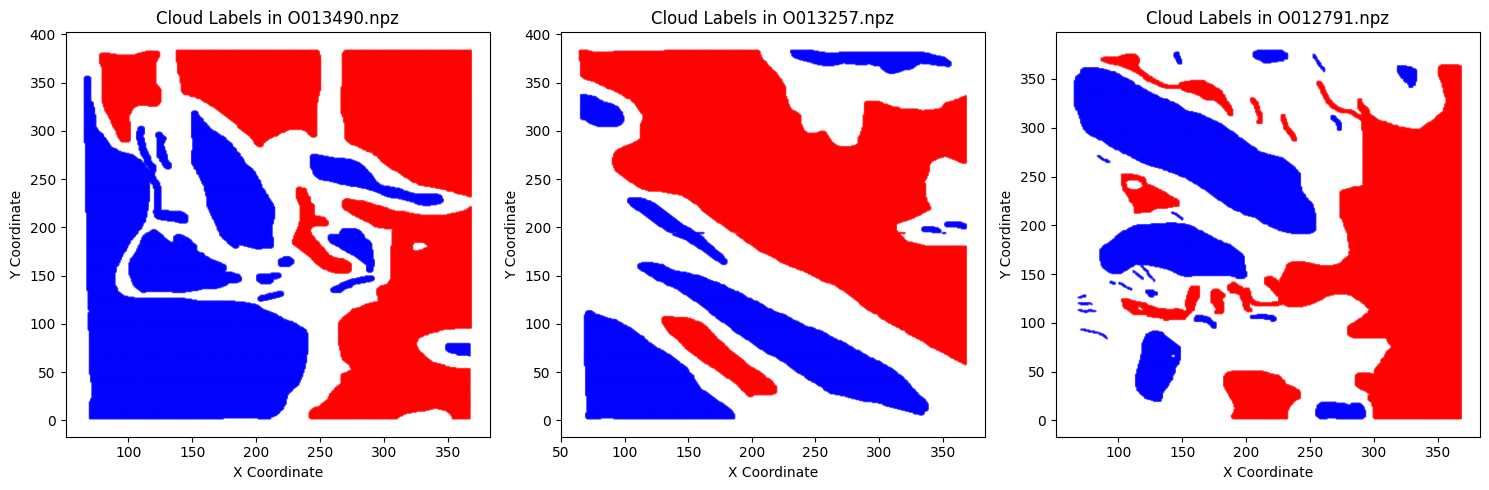
\includegraphics[width=0.8\textwidth]{labeled_cloud.png}
    \caption{Cloud labels}
    \label{Figure 1}
\end{figure}

To better understand the relationship between cloud presence and radiance values across different viewing angles, we conducted an exploratory analysis of the dataset. The radiance distributions from five angles (DF, CF, BF, AF, AN) for different orbits are visualized in Figure X, while the corresponding cloud labels are shown in Figure 2, 3, 4.

\begin{figure}[H]
    \centering
    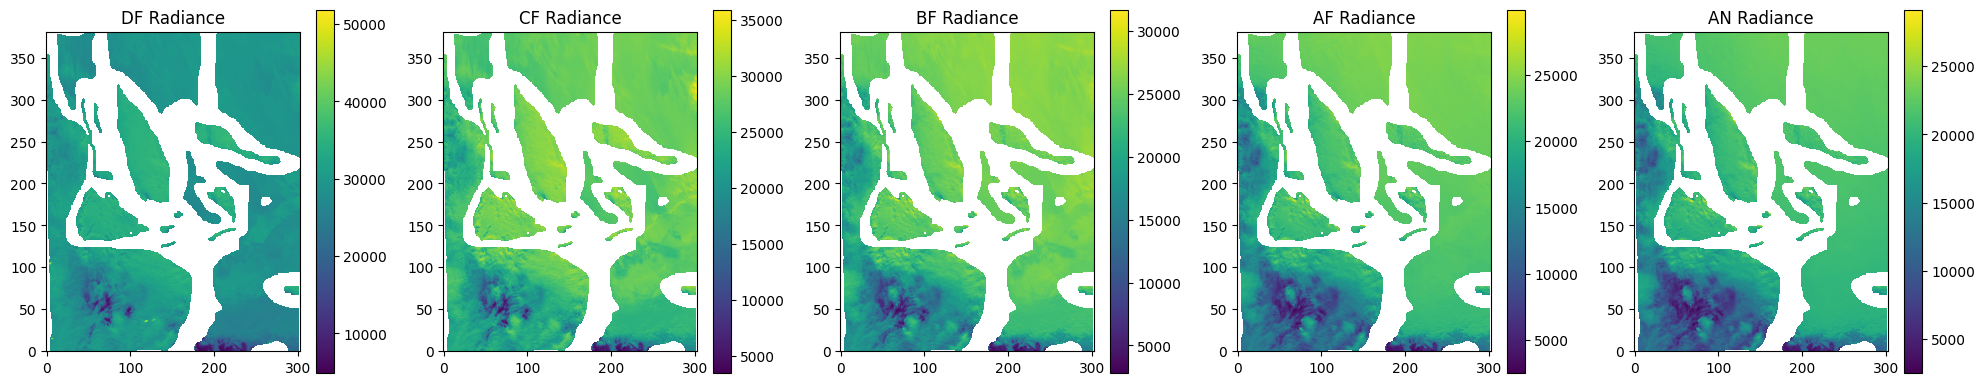
\includegraphics[width=0.8\textwidth]{radiance_O013490.png}
    \caption{Radiance of O013490}
    \label{Figure 2}
\end{figure}

\begin{figure}[H]
    \centering
    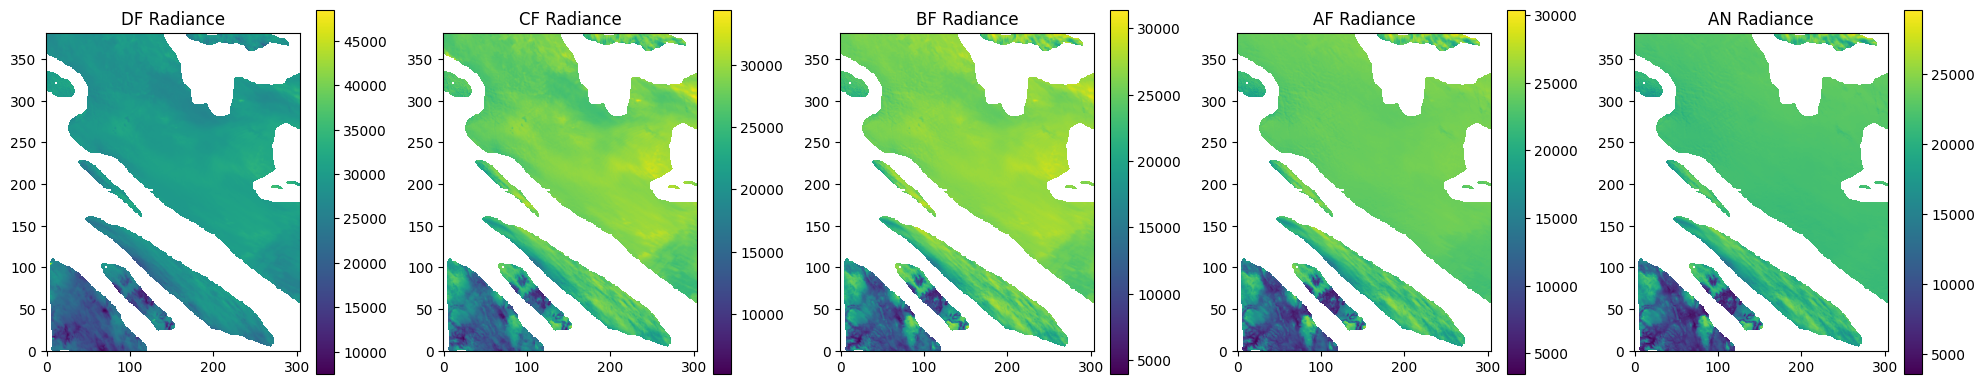
\includegraphics[width=0.8\textwidth]{radiance_O013257.png}
    \caption{Radiance of O013257}
    \label{Figure 3}
\end{figure}

\begin{figure}[H]
    \centering
    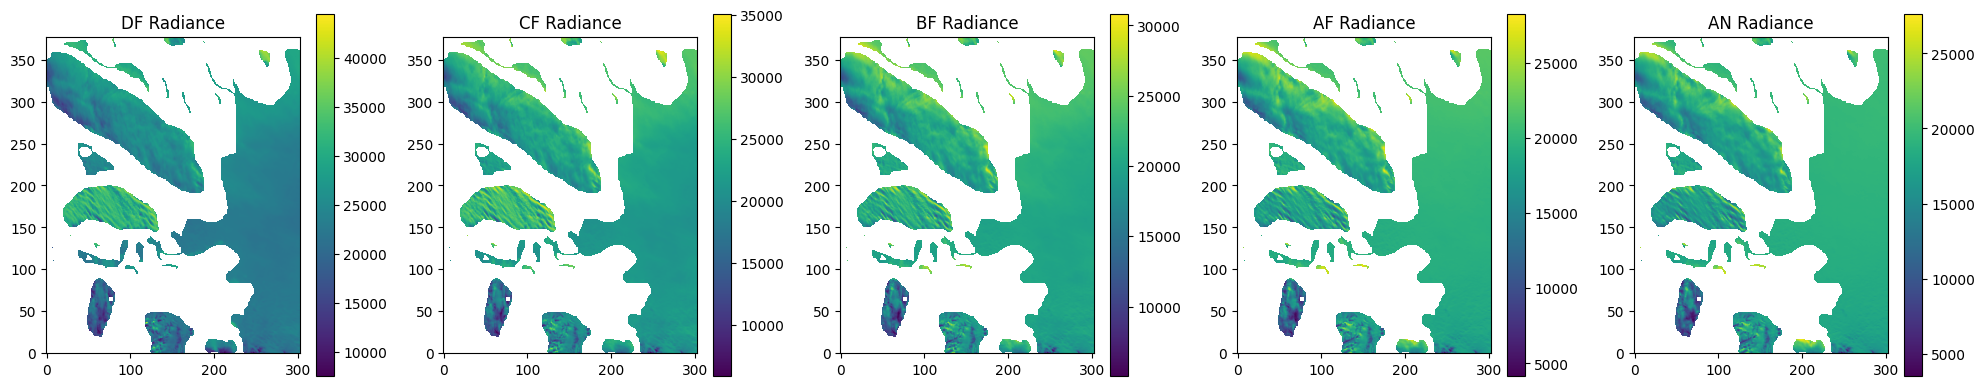
\includegraphics[width=0.8\textwidth]{radiance_O012791.png}
    \caption{Radiance of O012791}
    \label{Figure 4}
\end{figure}

Figure 1-4 reveals that cloud-covered regions tend to exhibit lower radiance values than non-cloud regions. This suggests that the measured spectral bands are likely in the thermal infrared (TIR) range,  where Clouds appear colder than the ground, emitting less thermal radiation. Non-cloud regions (such as land and ocean) tend to retain and emit more heat, resulting in higher radiance values.

The boxplot of the MISR cameras in Figure 5 shows that the distributions of radiance measurements across all angles are fairly similar, mostly ranging between 10,000 and 50,000. The boxplot also reveals a clear decreasing trend in radiance measurements as the camera angle decreases. This happens because, at larger angles, electromagnetic signals travel a longer distance before being captured by the sensor, leading to higher radiance measurements due to the extended atmospheric path and exposure.

Specifically, cameras Df, Cf, Bf, Af, and An take images at angles of 70.5°, 60.0°, 45.6°, 26.1°, and 0°, respectively. In this order, it is evident that the median radiance measurements decrease with decreasing angle, with Df (70.5°) showing the largest measurements and An (0°) the smallest.

Additionally, the spread of the data appears consistent across cameras and does not exhibit any extreme outliers. This is useful because it suggests that the data is mostly clean and ready for analysis.

\begin{figure}[H]
    \centering
    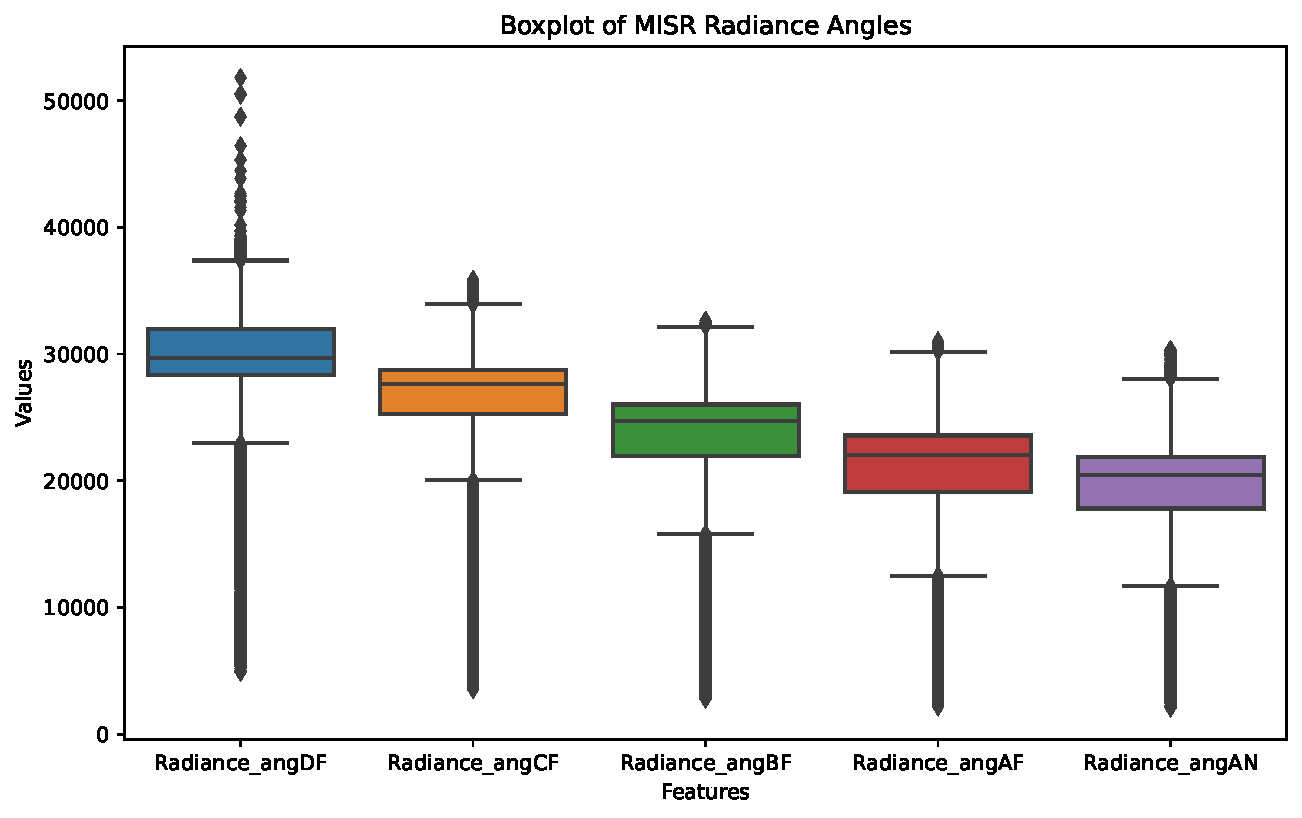
\includegraphics[width=0.8\textwidth]{my_boxplot.pdf}
    \caption{Distributions of MISR Radiance Angles}
    \label{Figure X}
\end{figure}

We also explore the three main features used in the authors’ paper: CORR, SD, and NDAI. The distributions for these features are shown in Figure 6, stratified into two groups — cloud and no-cloud pixels — based on expert labeling. The data for this EDA comes from three MISR images where each pixel has been labeled as cloud or no cloud by experts.

In Section 3.0 (Feature Engineering), we take a closer look at these distributions to help establish threshold values for classification modeling using ELCM-QDA (Enhanced Linear Correlation Matching – Quadratic Discriminant Analysis) and other techniques.

In cloud detection tasks using satellite imagery, the Normalized Difference Angular Index (NDAI) is commonly used to distinguish between cloud and non-cloud pixels. To enhance the feature representation, we introduce a gradient-based transformation of NDAI, which captures the spatial variations across different regions. The goal of this transformation is to highlight local intensity changes, which could be useful for edge detection and improving classification models. 


\begin{figure}[H]
    \centering
    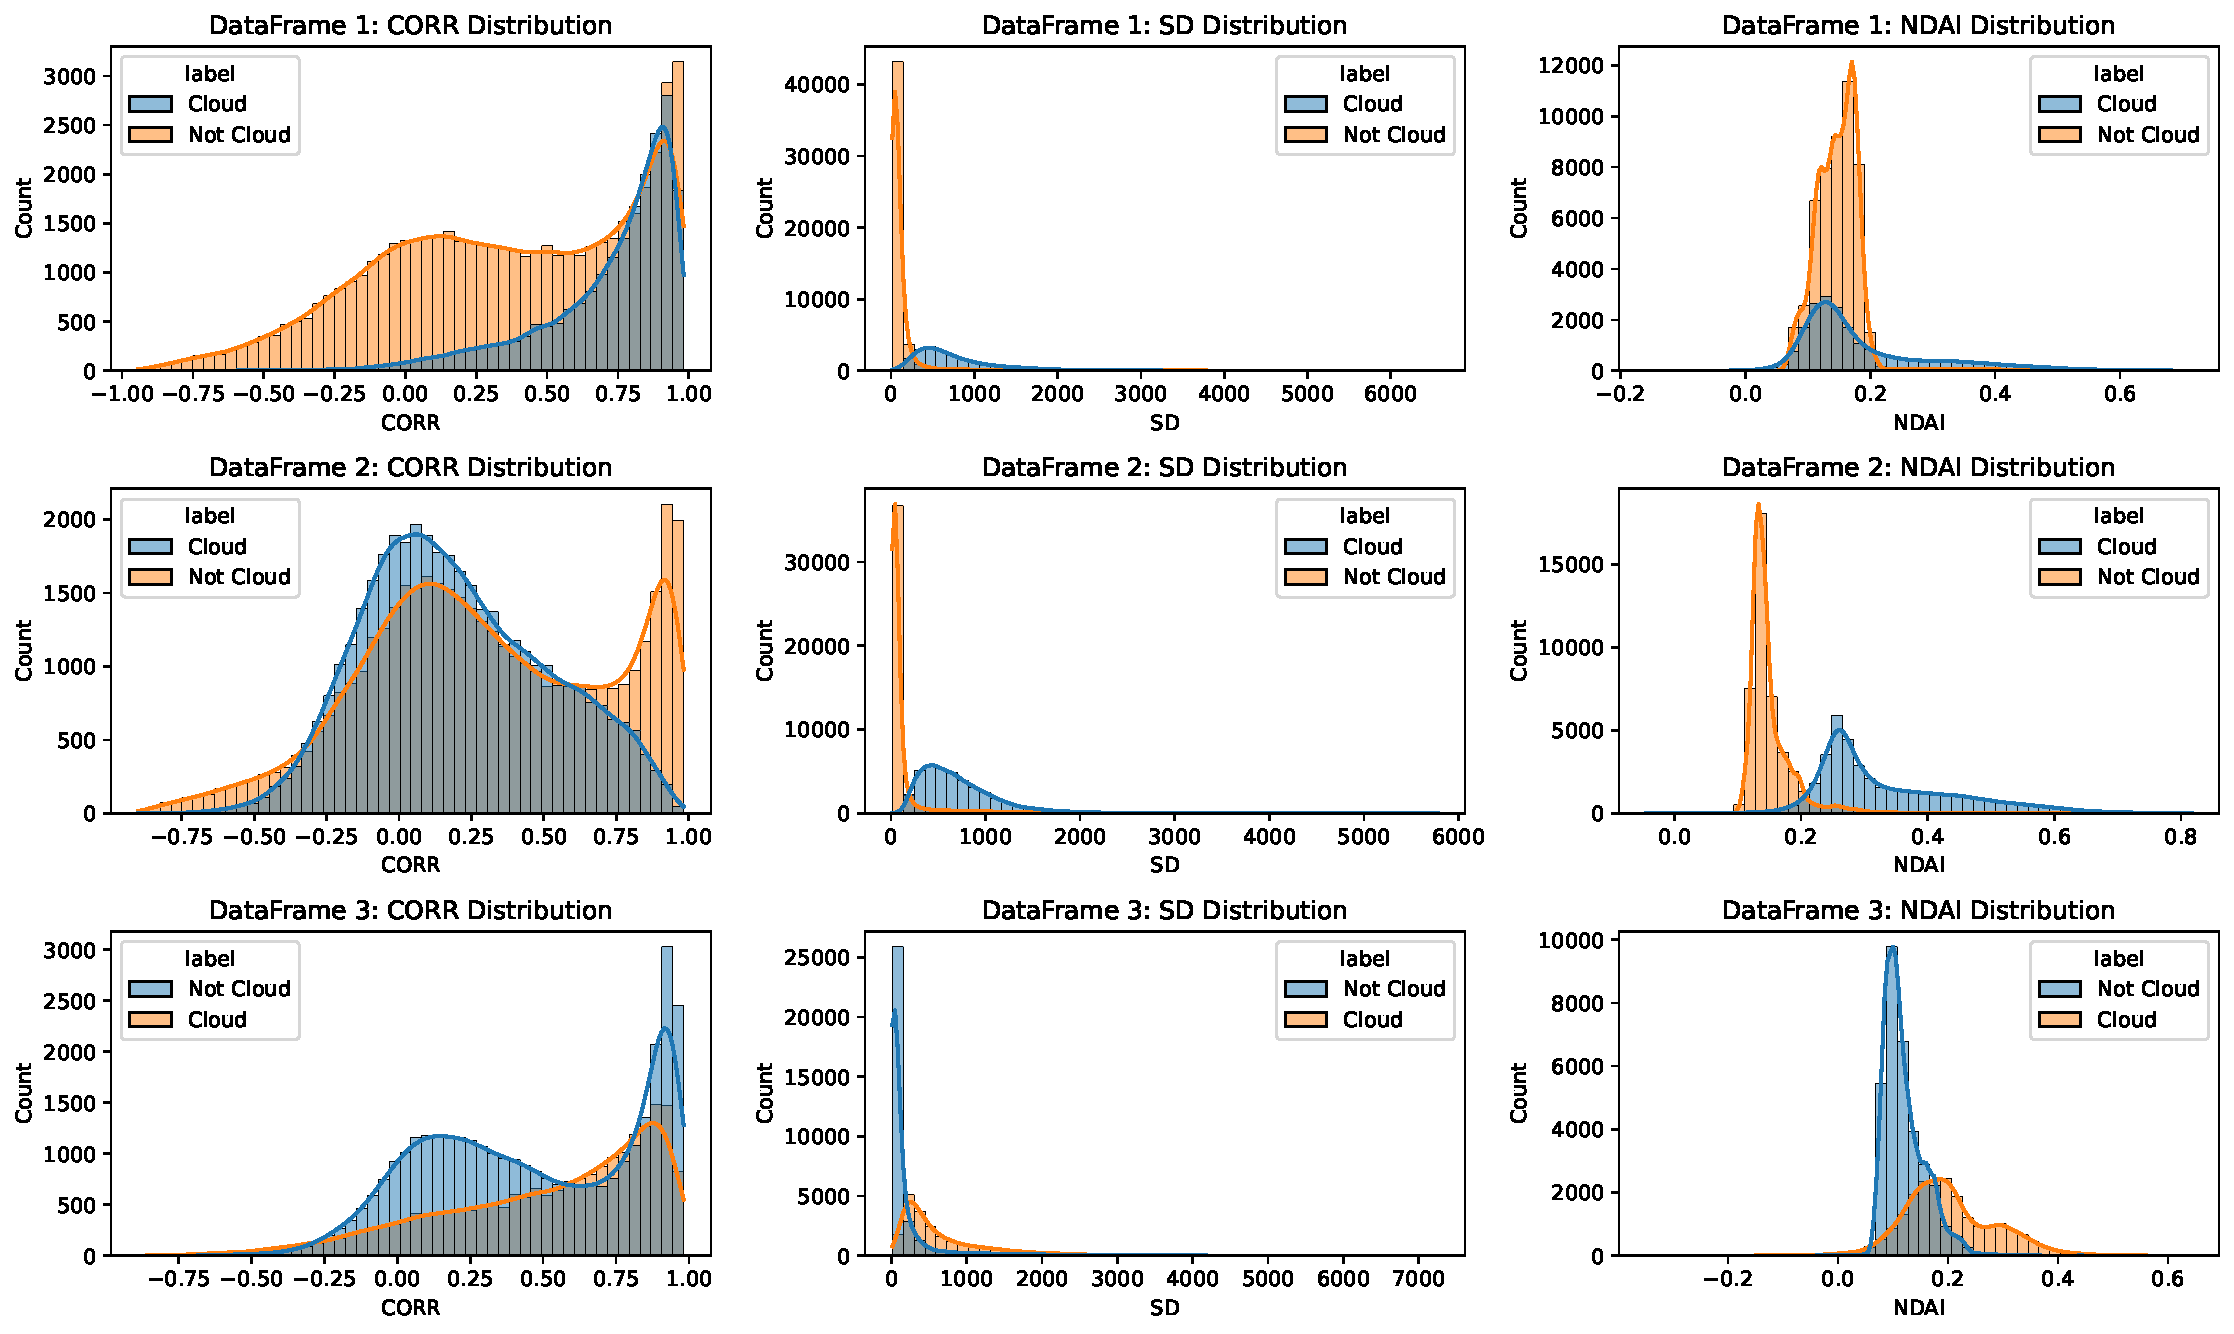
\includegraphics[width=0.8\textwidth]{my_plot_features.pdf}
    \caption{Histogram Distributions of CORR, NDAI, and SD: Clouds vs. No Clouds}
    \label{Figure X}
\end{figure}

This result also provide intuitive support for the usefulness of NDAI, which is defined as (DF-AN)/which is calculated based on the difference between DF and AN, normalized by their sum to account for overall intensity variations.

As shown in Figure 2-4, cloud regions tend to exhibit systematically lower radiance values than non-cloud regions, particularly in DF and AN angles. This suggests that the angular dependency of radiance can be leveraged to differentiate clouds from non-cloud regions. 

\begin{figure}[H]
    \centering
    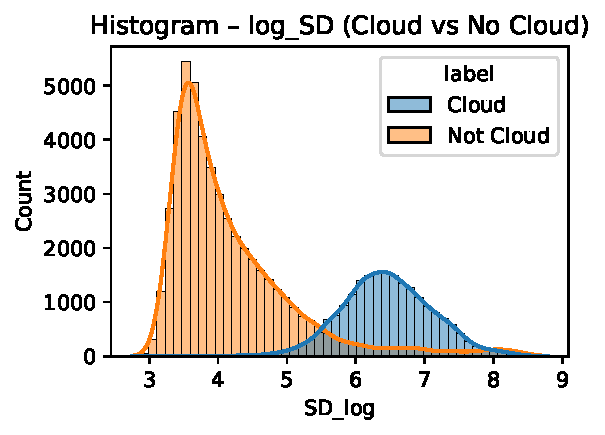
\includegraphics[width=0.8\textwidth]{sd_log_fig.pdf}
    \caption{Histogram Distribution Log SD: Clouds vs. No Clouds}
    \label{Figure X}
\end{figure}

\section{Feature Engineering}

\subsubsection{ELCM-QDA Feature Engineering}

For our ELCM-QDA cloud classification model, we began with the same three core features used by the authors. ELCM-QDA requires threshold values that split the feature data into distinct groups. By examining Figure 6, we determined that a CORR threshold of 0.75 was appropriate, as it marks a clear divergence between cloud and non-cloud labeled pixels. This also aligns with the threshold used in the original paper.

The SD distribution was heavily left-skewed, making it difficult to visually select a threshold. We applied a logarithmic transformation, and the threshold for “Log SD” became clearer at around 5.5 in Figure 7. We confirmed this threshold through grid search optimization, the same approach used for NDAI.

For NDAI, visual inspection wasn’t sufficient, so we also used grid search. The thresholds identified for the three images were 0.243, 0.157, and 0.178, all falling within the 0.08–0.40 range reported in the paper, validating our approach for the ELCM-QDA model.


\subsection{New Feature Engineering}

\subsubsection{Alternative NDAIs}

Based on our findings from the EDA, we initially experimented with different variations of NDAI to explore potential improvements. The radiance distribution heatmaps (Figure 2-4) suggest that DF exhibits a relatively small difference between cloud and non-cloud regions, making it a suitable choice as the normalization variable in the NDAI formula rather than a feature to be replaced.

Given this, we explored alternative NDAI by replacing AN with other radiance measurements (e.g., AF, BF, or CF) to see if different angular combinations would improve cloud differentiation. Through this approach, we derived three alternative NDAI formulations: NDAI\_AF, NDAI\_BF, and NDAI\_CF, each replacing AN with AF, BF, and CF, respectively. 

\subsubsection{Spatial Gradients of NDAIs}

To enhance NDAI's ability to differentiate between cloud and non-cloud regions, we introduce gradient-based features, which quantify the spatial variation of NDAI across different regions. By computing the NDAI gradients along both horizontal and vertical axes, we aim to capture edge characteristics and local transitions between cloud and non-cloud areas.

The gradient is derived through the following steps:

\textbf{Step 1: Computing Gradients}  

To capture local variations, we compute the spatial gradients of NDAI in both horizontal (\( x \)) and vertical (\( y \)) directions. The gradients are obtained using partial derivatives. Let \( G_x \) and \( G_y \) represent the gradient components along the \( x \)- and \( y \)-axes, respectively. In practice, we use neighboring pixels to estimate these derivatives.

\textbf{Step 2: Computing Gradient Magnitude}  

The overall magnitude of the gradient at each pixel \( G \) is obtained by combining the horizontal and vertical components using the Euclidean norm. This measures the total intensity of the change in NDAI at a given location.

\textbf{Step 3: Applying Log Transformation}  

The raw NDAI gradient magnitude exhibits a highly skewed distribution, making it difficult to establish a clear threshold for distinguishing between cloud and non-cloud regions. As shown in Figure 5, the majority of values are concentrated near zero, with a long tail extending towards larger values. This makes it challenging to set an effective decision boundary.

\begin{figure}[H]
    \centering
    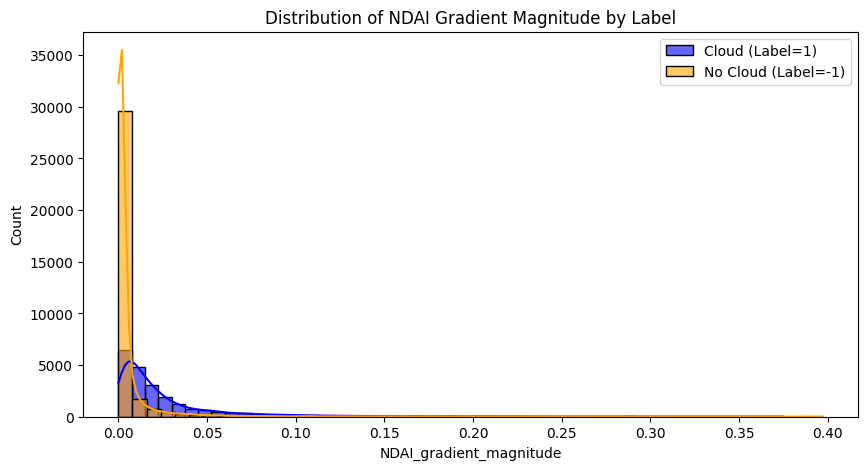
\includegraphics[width=0.8\textwidth]{dist_of_NDAI_grad.png}
    \caption{Distribution of NDAI Gradient Magnitude by Label}
    \label{Figure 5}
\end{figure}

To address this issue, we apply a logarithmic transformation to the NDAI gradient magnitude plus \( \varepsilon  \), where \( \varepsilon = 10^{-6} \) is a small constant added to prevent numerical instability when \( G \) is zero.

After applying the logarithmic transformation, the feature distribution becomes more Gaussian-like, and a clear separation between cloud (Label=1) and non-cloud (Label=-1) regions emerges, as illustrated in Figure Y. Notably, the transformed feature allows for an effective threshold of -5, where most cloud pixels fall above this value, and non-cloud pixels fall below. This suggests that log-transformed NDAI gradient magnitude provides a more discriminative representation for cloud classification.

\begin{figure}[H]
    \centering
    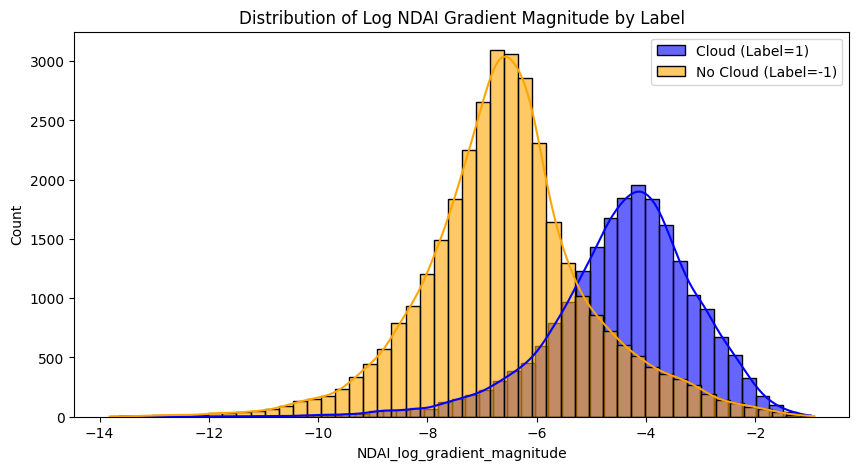
\includegraphics[width=0.8\textwidth]{dist_of_log_NDAI_grad.png}
    \caption{Distribution of log NDAI Gradient Magnitude by Label}
    \label{Figure 6}
\end{figure}

These observations highlight the advantage of applying logarithmic scaling to gradient-based features, particularly in cases where raw gradient values are highly skewed. The improved separability makes this transformed feature a strong candidate for inclusion in classification models.

\subsection{Transfer Learning}

In this section, we first fit the autoencoder on the 161 unlabeled images, then fine-tune our dataset on the training set of 3 labeled images. Finally, with the fixed autoencoder, we can get the eight autoencoder feature embedding for all image data, while we will specifically use the autoencoder feature embedding for the 3 labeled images.

\subsubsection{Data Preprocessing for Autoencoder}

To prepare the training dataset for the pre-trained autoencoder, we will process 161 unlabeled satellite images. The main process for this stage is in python file \textit{data.py} and \textit{patchdataset.py}. 



Each image file contains pixel-level data, including spatial coordinates (x, y) and 8 feature channels (NDAI, SD, CORR, and 5 radiation angles). We first excluded three expert-labeled images to ensure that autoencoder training remained completely unsupervised. After reshaping, we apply global normalization. This improves training stability and speeds up convergence. For each valid pixel, we extract a 9×9 patch centered on that point, including all 8 feature channels. To handle edge cases, we fill the image with reflections. These patches will be the training samples for the autoencoder. Finally, we created a custom PyTorch PatchDataset class to efficiently load patches.


This pre-processing step provides a large and standardized patch dataset for unsupervised feature learning for our autoencoder.

\subsubsection{Autoencoder Architecture and Training}

The autoencoder was implemented using PyTorch Lightning, and it takes 9×9 patches of input data generated in the last stage. The goal is to reconstruct each input patch and minimize the reconstruction error.

The core setting of the autoencoder is saved in the file \textit{autoencoder.py}. The training script, which serves as the primary function of this stage, is located in \textit{run\_autoencoder.py}. In the \textit{configs} folder, we save detailed parameters and file path settings for model training, such as in \textit{default.yaml}. The top-performing model checkpoints are saved in the \textit{checkpoints} directory. Since model training can be time-consuming, we submit the job using a Slurm batch script (\textit{job.sh}) for efficient computation. All outputs, including logs, errors, and loss records, are saved in the \textit{log} folder.


\textbf{Model Architecture}

The model consists of two parts: an encoder and a decoder. The encoder flattens the input patch and passes it through three fully connected layers with ReLU activations. The final output of the encoder is an embedding vector of size 8. The decoder mirrors this structure, transforming the embedding back into the original input shape.

Specifically, the architecture is defined as follows:

\textbf{Encoder:}

\begin{itemize}
    \item Input size: $8 \times 9 \times 9 = 648$
    \item Linear(648 $\rightarrow$ 128) $\rightarrow$ ReLU
    \item Linear(128 $\rightarrow$ 64) $\rightarrow$ ReLU
    \item Linear(64 $\rightarrow$ 8)
\end{itemize}


\textbf{Decoder:}

\begin{itemize}
    \item Linear(8 $\rightarrow$ 64) $\rightarrow$ ReLU
    \item Linear(64 $\rightarrow$ 128) $\rightarrow$ ReLU
    \item Linear(128 $\rightarrow$ 648) $\rightarrow$ Unflatten to (8, 9, 9)
\end{itemize}

\textbf{Training Details}

We used Mean Squared Error (MSE) loss between the input and the reconstructed patch. The optimizer was Adam with a learning rate of 0.001. Training was conducted for up to 50 epochs, with early stopping based on validation loss. The batch size was set to 4096, and we used 4 workers to speed up data loading.
We monitored both training and validation loss during training. For each run, we save the top 3 best-performing models (smallest validation errors) into the folder Checkpoints. All experiments were recorded with lightening for better tracking and comparison, and the results are saved in the \textit{log} folder.

Here is a summary of part of the training configuration:

\begin{itemize}
\item Patch size: 9
\item Batch size: 4096
\item Embedding size: 8
\item Max epochs: 50
\item Early stopping: patience = 10, monitor = val\_loss, delta = 0.001
\item Learning rate: 0.001
\end{itemize}


Based on the rough autoencoder fitting outcome, we can get the best model (smallest validation errors). Then based on this model, we can begin fine-tuning the model on the 3 labeled image. 

\subsubsection{Finetuning}

After we have got the best-trained autoencoder on 161 unlabeled images, we will finetune our model on the training sets of the three labeled images.  We add new functions and classes in textit{data.py} and \textit{patchdataset.py}. The difference is that we must pass labels into the model for supervised learning in this step. In this data preprocessing part, we extracted 9×9 patches centered on each valid pixel from the three labeled images, and only pixels with expert labels (+1 or -1) were used.


We developed the \textit{fine\_tuning.py} for the core part of finetuning. For the supervised learning, we develop a new module \textit{AEClassifier} to wrap the frozen encoder and a simple fully connected layer (Linear(8, 1)) that maps the 8-dimensional latent representation to a binary output. Then during training, we use the \textit{BCEWithLogitsLoss} function to handle binary classification. Labels are preprocessed into +1/-1 and converted to 0/1 targets in the loss computation. 

The fine-tuning process was also implemented using PyTorch Lightning. The optimizer is still Adam, and we switch to a smaller learning rate at 0.0001 and a smaller Max Epoch at 20. We still use early stopping and model checkpointing to monitor the validation loss.

To sum up, the key differences of \textit{fine\_tuning.py} from the original \textit{run\_autoencoder.py} include:

\begin{itemize}
\item  Use a training set of labeled data only, instead of all 161 images.
\item Change the loss function from MSE to binary cross entropy loss.
\item Using labeled pixel values as supervised targets, rather than unsurpervised learning in last step
\end{itemize}


The training logs were then stored in \textit{finetune} folders. The loss shows that both training and validation loss decrease across epochs, which indicate that the autoencoder benefit from light finetuning. Finally, with the rough training on unlabled dataset and finetuning on labled dataset, we can have our model fixed and look into the best autoencoder.



\subsubsection{Model Loss Analysis}



We store our best model in the checkpoint folder, the detailed file path is \textit{checkpoints/exp\_0316/exp-epoch=036-val\_loss=0.1052.ckpt}. This file contains all the detailed training parameters and training details for this model. The corresponding loss analysis is also stored in \textit{logs/autoencoder/version\_6/metrics.csv}. 

Based on the training outcome, with the Max Epoch set as 50, the autoencoder early stops at the 36th epoch, 134347 steps. The final validation loss drops to 0.1052. 

We store the training loss for each step and the validation loss for each epoch. That's why the validation loss is smoother in the figure, as the data points are much fewer than the training loss. We can see that both training and validation loss drops quickly to below 0.12 within the first epoch. Then the training loss for each step varies within the level of validation loss for each epoch. The loss kept decreasing slightly, and early stopping was finally called at the 36th epoch.

\begin{figure}[H]
    \centering
    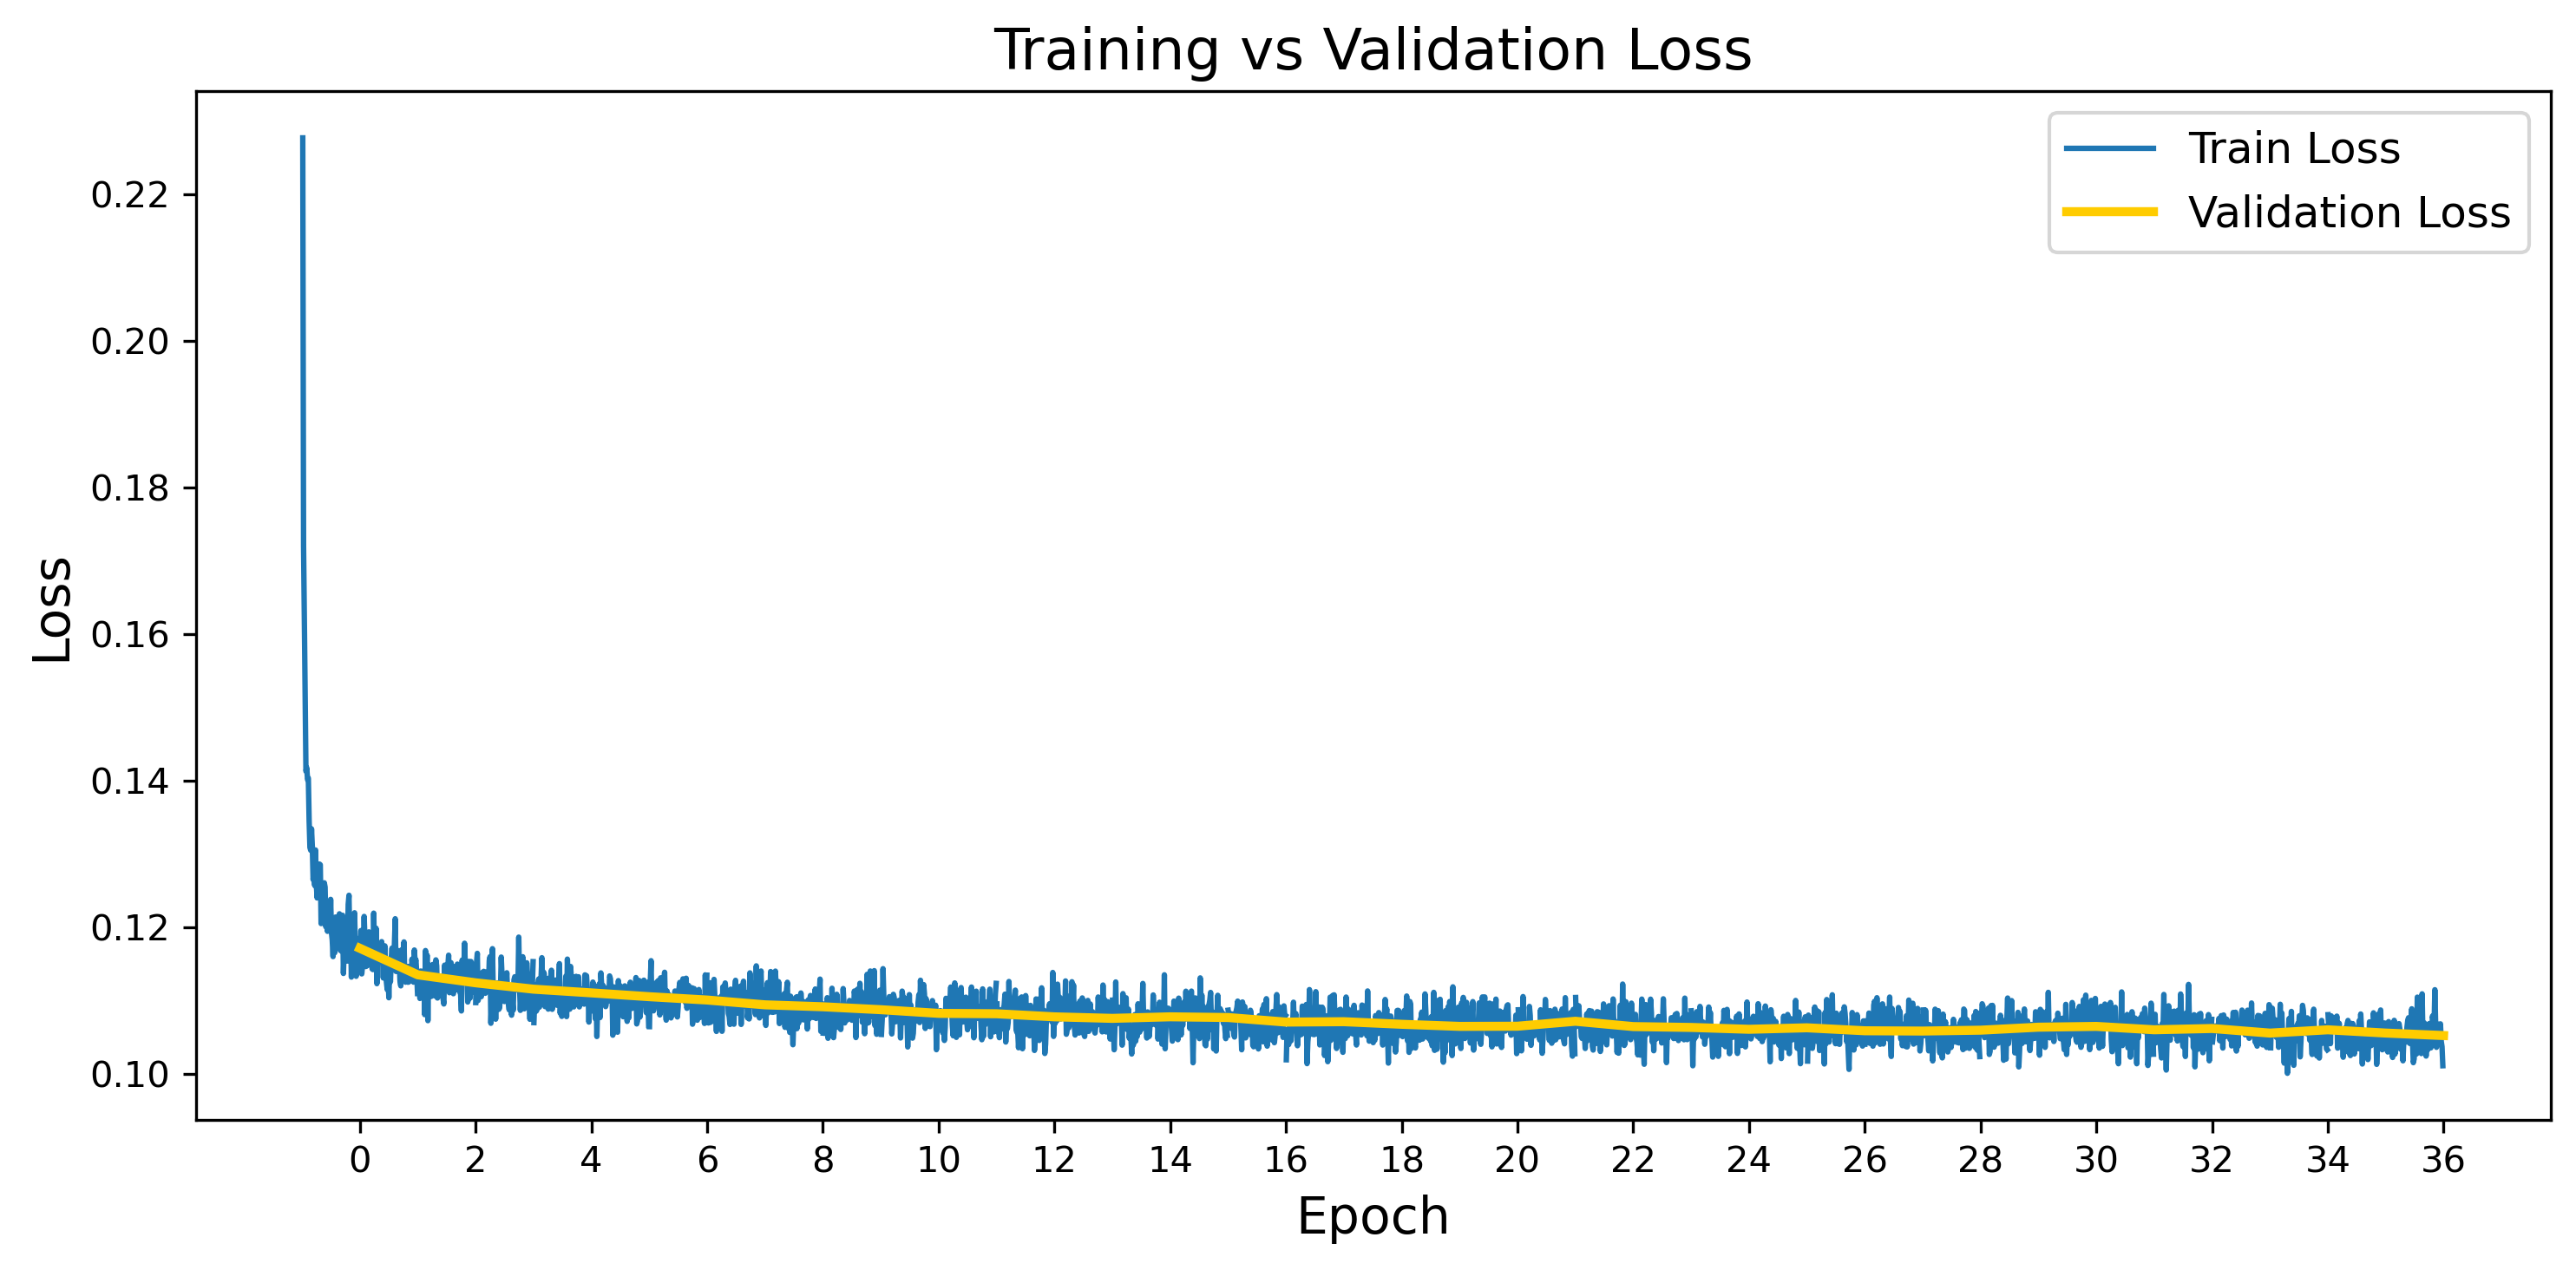
\includegraphics[width=0.95\textwidth]{loss_plot.png}
    \caption{Autoencoder Training and Validation Loss Across Epoch}
    \label{Figure 7}
\end{figure}

Based on the loss analysis, we can conclude that this autoencoder has been well-fitted. Therefore, we can move to the final part, calculating the embedding with this best embedding.



\subsubsection{Feature Embedding}


The core code for generating the feature embedding is in the \textit{get\_embedding.py}. To speed up the calculation, we also create a Slurm batch script (\textit{job\_embedding.sh}) for efficient computation. In this step, we use the best autoencoder we selected to extract embeddings from the 164 images. We will load the model checkpoint and apply the encoder to every 9×9 patch generated in the preprocessing stage.

For each image, we computed the 8-dimensional embedding for each valid pixel and saved the results as CSV files. Each output file contains the pixel coordinates (y, x) and the corresponding embedding features (ae0 to ae7). Files for the three labeled images (image 15, image 17, image 18) will be used as additional features in the modeling part. Here, images 15, 17, and 18 correspond to the original image [O012791, O013257, O013490] by order. The AE features dataset can be matched with original dataset based on the first two columns x and y.

To check the embeddings and their general relation with the true label, we consider Principal Component Analysis on the 8 AE features. We take Image 17 in folder \textit{Outcome\_3\_image\_2} as an example. After we had done PCA on the 8 AE features, we visualized the first two PC. From the figure, the red (-1.0) cluster is mainly located tightly on the left side, and the blue (1.0) clusters span across the right side of the figure. This indicates feature separations and suggests that the autoencoder effectively captures class differences. However, the true effects of AE features in label prediction need to be studied in the modeling part.

\begin{figure}[H]
    \centering
    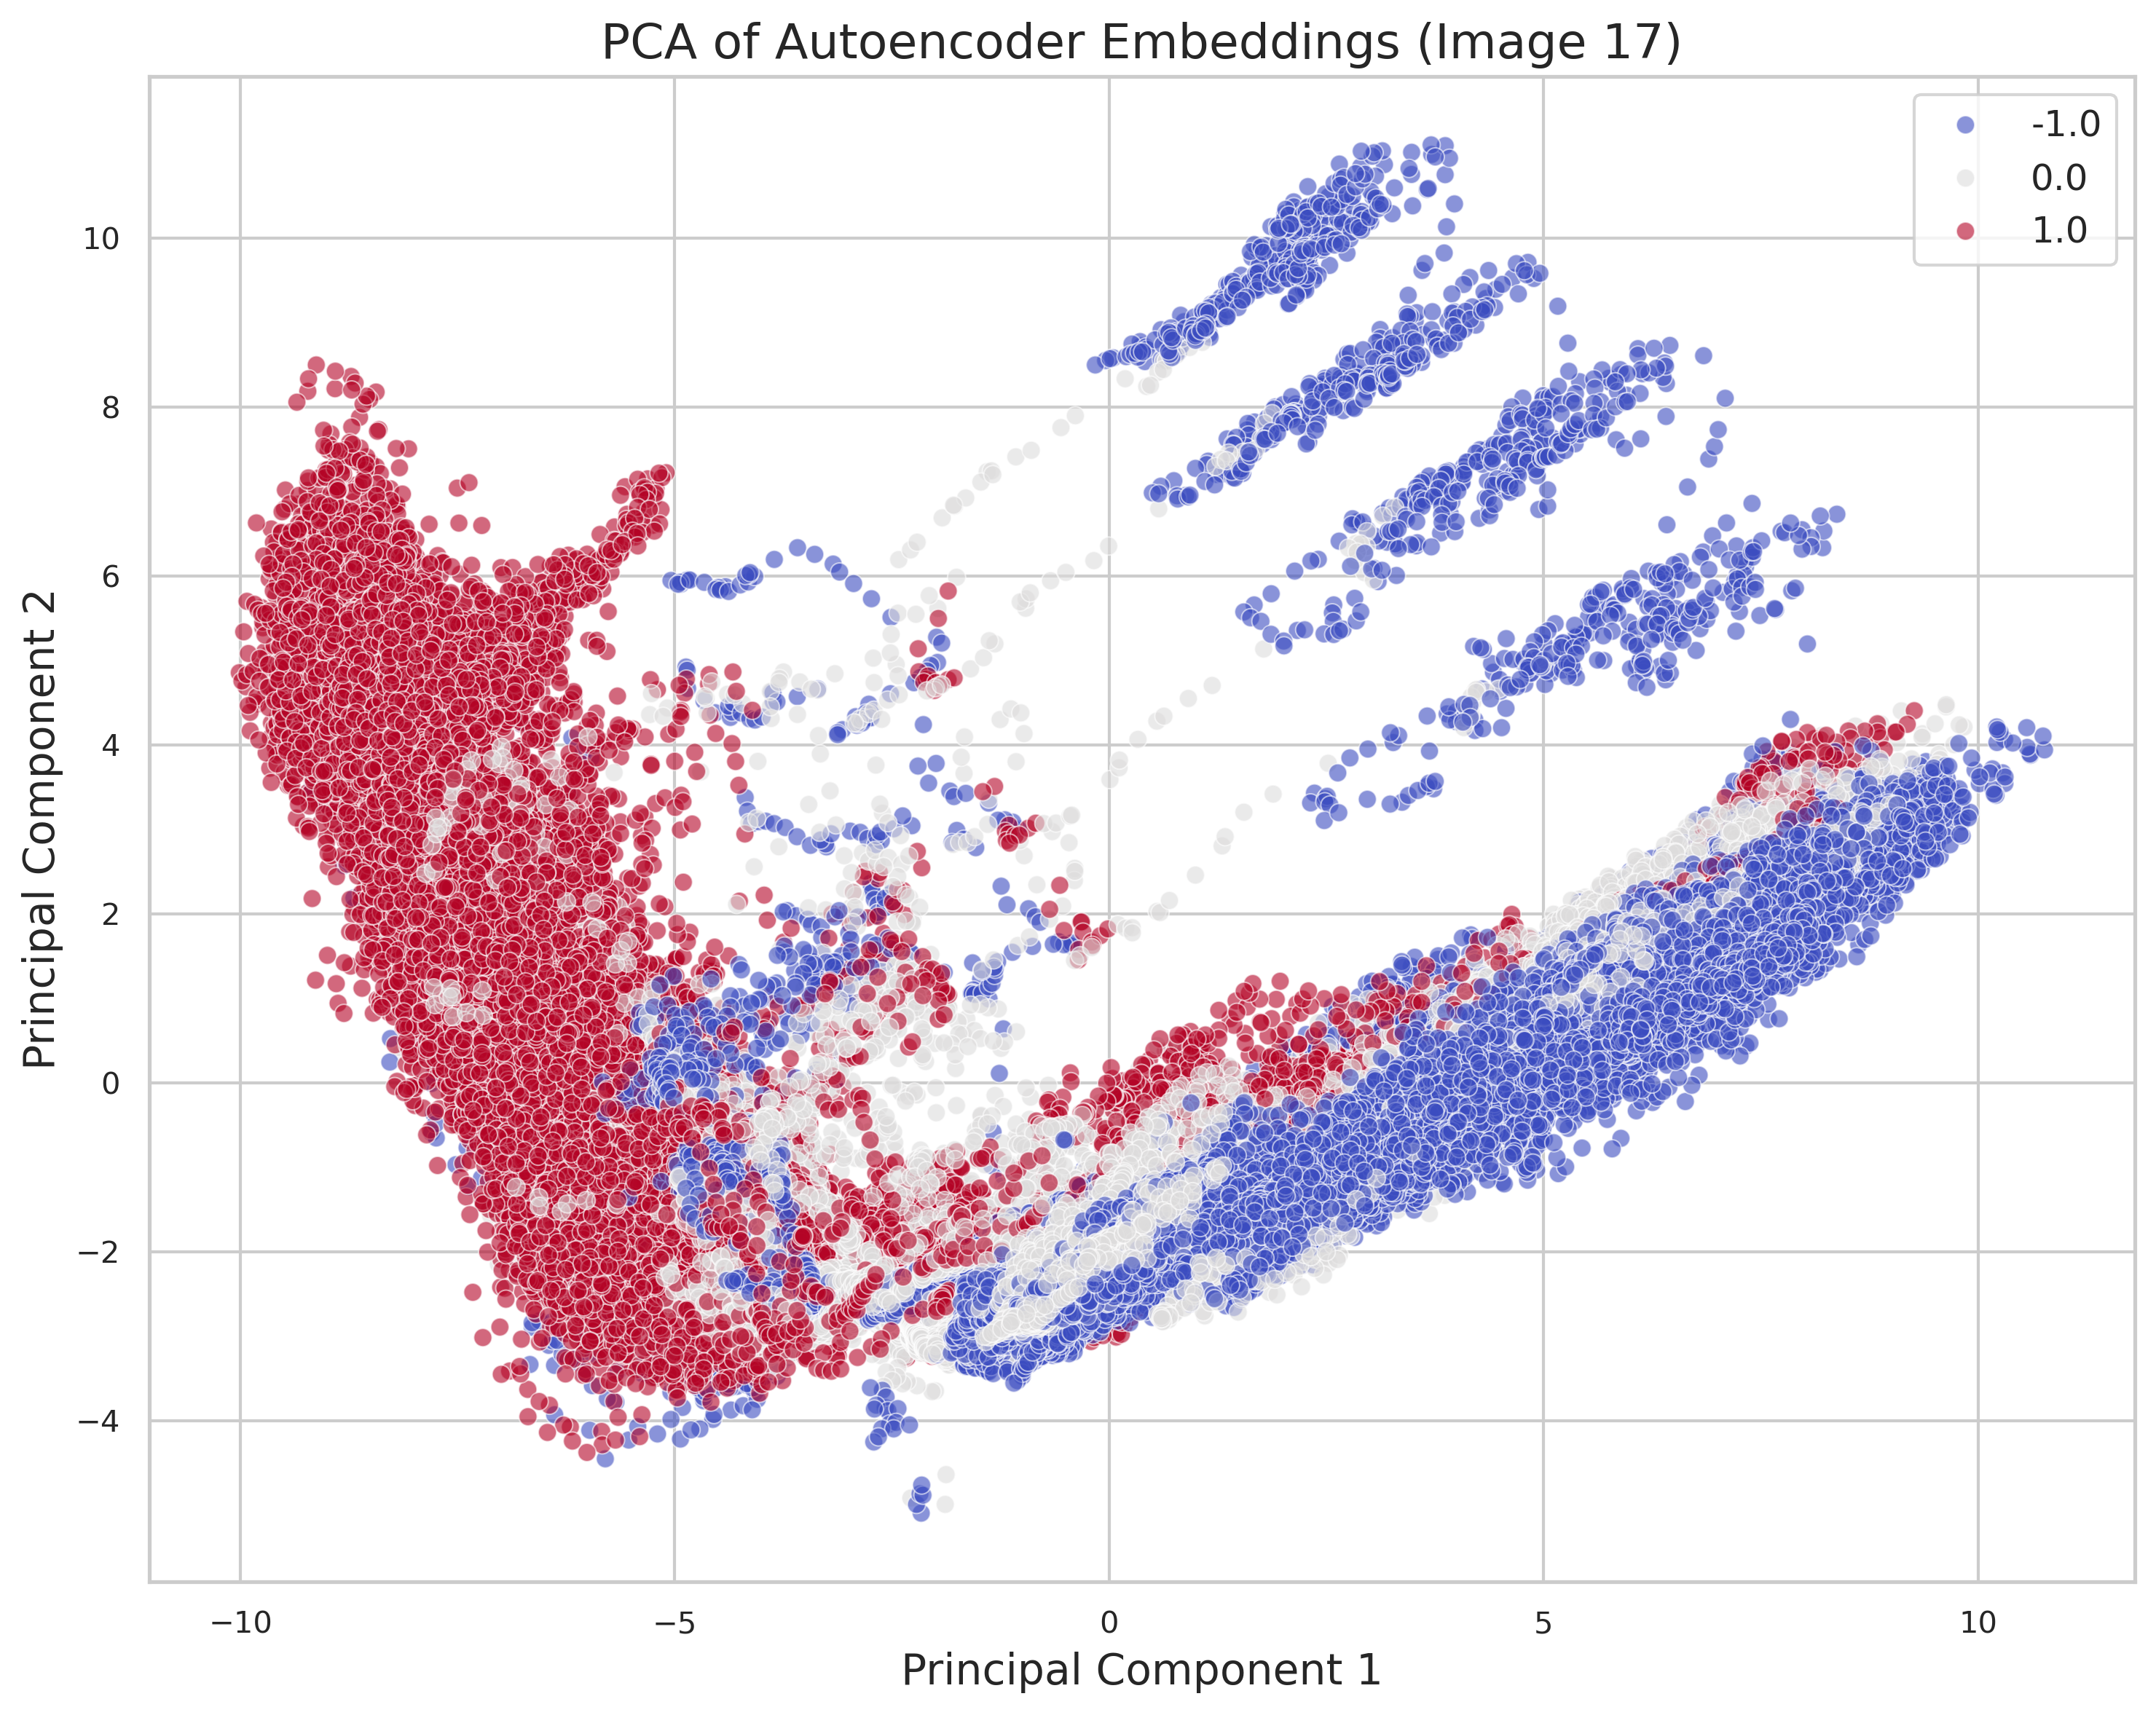
\includegraphics[width=0.8\textwidth]{AE_features.png}
    \caption{First Two Principal Components of Eight AE Features, Image 17 (O013257)}
    \label{Figure 8}
\end{figure}















\section{Modeling}
 This section presents the four classification models developed for cloud detection in polar regions. For each model, we describe the algorithm, its implementation details, the underlying assumptions, and our methods for testing these assumptions. The models range from simpler linear approaches to more complex nonlinear techniques, allowing us to explore different trade-offs between interpretability and predictive performance. Our systematic testing of model assumptions ensures that the selected classifiers are appropriate for the cloud detection task and can reliably distinguish between cloud and non-cloud pixels.

 \subsection{Model Overview}
 
\subsubsection{Logistic Regression}

\textbf Logistic regression is a probabilistic linear classification algorithm that models the probability of cloud presence using the logistic (sigmoid) function. For our cloud detection task, the model computes:

\begin{equation}
P(cloud | x) = \frac{1}{1 + e^{-(\beta_0 + \sum_{i=1}^{n} \beta_i x_i)}}
\end{equation}

where $\beta_i$ represents the learned coefficient for feature $x_i$. The model predicts a pixel as a cloud when this probability exceeds 0.5. We implemented logistic regression with L2 regularization (penalty parameter C=1.0) and balanced class weights to mitigate the impact of the class imbalance in our dataset (61\% non-cloud vs. 39\% cloud pixels). Logistic regression's primary advantage is its interpretability. The coefficients directly indicate each feature's contribution to the prediction.

Assumptions:
\begin{enumerate}
    \item Linear relationship between features and log odds of the outcome
    \item Independence of observations
    \item No severe multicollinearity among predictors
    \item No extreme outliers
\end{enumerate}

Testing Assumptions:
To test the linearity assumption, we examined the relationship between continuous features and the logit of cloud probability. Most features showed approximately linear relationships with the log odds, though some (particularly NDAI and its derivatives) exhibited slight nonlinearity at extreme values. This may explain why logistic regression, while performing well (AUC 0.967), couldn't match the performance of nonlinear models.

Residual analysis showed no systematic patterns, and the model achieved balanced precision (0.87) and recall (0.92) for cloud detection, indicating a reasonable fit to the data despite the simplifying linear assumption.

\subsubsection{Support Vector Machine (SVM)}

Support Vector Machine (SVM) is a powerful classification algorithm that finds an optimal hyperplane to maximize the margin between cloud and non-cloud pixels in feature space. The decision function for SVM is:

\begin{equation}
f(x) = \sum_{i=1}^{n} \alpha_i y_i K(x_i, x) + b
\end{equation}

where $\alpha_i$ are the learned weights, $y_i$ are the class labels, $K$ is the kernel function, and $b$ is the bias term. 

Our implementation used a Radial Basis Function (RBF) kernel to transform the data into a higher-dimensional space:

\begin{equation}
K(x_i, x_j) = \exp(-\gamma ||x_i - x_j||^2)
\end{equation}

The hyperparameters C=10 and gamma=0.01 were selected through grid search cross-validation. The C parameter controls the trade-off between achieving a low training error and a low testing error (regularization), while gamma defines the influence radius of each training example. Due to computational constraints with our large dataset ($\sim$200,000 pixels), we used a randomly selected subset of 10,000 training samples for model fitting.

Assumptions:
\begin{enumerate}
    \item The classes are separable in the feature space transformed by the kernel
    \item The RBF kernel appropriately captures the data's nonlinear structure
    \item The regularization parameter C appropriately balances margin maximization and error minimization
    \item Features have comparable scales (particularly important for distance-based algorithms like SVM)
\end{enumerate}

Testing Assumptions:
Standard scaling was applied to all features to meet the fourth assumption. The high AUC score (0.990) suggests that the RBF kernel successfully transformed the data into a space where clouds and non-clouds are highly separable. 

We validated the separability assumption by visualizing the distribution of decision function values, which showed clear separation between the classes. The effectiveness of the RBF kernel was confirmed by comparing performance against linear and polynomial kernels, with RBF consistently outperforming alternatives by 2-3\% in validation AUC.

The precision (0.94) and recall (0.96) metrics for cloud detection confirm that both classes are well-classified with minimal bias toward either class. The SVM model's strong performance validates our kernel choice and hyperparameter selection, indicating that the model assumptions align well with the underlying data structure.

\subsubsection{XGBoost Classifier}

XGBoost (Extreme Gradient Boosting) is a sophisticated tree-based ensemble algorithm that builds decision trees sequentially, with each tree correcting errors made by previous trees. The prediction is given by:

\begin{equation}
\hat{y}_i = \sum_{k=1}^{K} f_k(x_i)
\end{equation}

where $f_k$ represents the $k$-th decision tree in the ensemble of $K$ trees. 

Our XGBoost implementation included 100 trees with a maximum depth of 6 nodes, a learning rate of 0.1 to control each tree's contribution, and row/column subsampling rates of 0.8 to increase model robustness and prevent overfitting. XGBoost offers several advantages for cloud detection, including capturing complex nonlinear patterns, handling interactions between features automatically, and providing interpretable feature importance metrics.

The model was trained using an objective function that combines both the logistic loss function and a regularization term:

\begin{equation}
L(\phi) = \sum_{i=1}^{n} l(y_i, \hat{y}_i) + \sum_{k=1}^{K} \Omega(f_k)
\end{equation}

where $l$ is the logistic loss function, and $\Omega$ is the regularization term that penalizes model complexity.

Assumptions:
\begin{enumerate}
    \item Features have varying importance levels for cloud detection
    \item Complex nonlinear relationships and interactions exist between features
    \item The ensemble approach can effectively reduce bias and variance
    \item The boosting process converges to an optimal solution
    \item The hierarchical splitting of the feature space by decision trees can effectively model the decision boundary between cloud and non-cloud regions
\end{enumerate}

Testing Assumptions:
Learning curve analysis showed consistent improvement in both training and validation AUC scores with diminishing returns after approximately 80-100 boosting rounds, confirming assumption 4. The final model achieved near-perfect discrimination (AUC 0.999) on both training and validation sets with a minimal gap between them, indicating appropriate model complexity without overfitting.

The stability analysis demonstrated exceptional robustness to input perturbations, with the model maintaining AUC scores above 0.995 even when random Gaussian noise (standard deviation 0.02) was added to test features. This strong stability confirms that the model captured genuine patterns rather than noise.

Feature importance analysis revealed significant variation in importance scores, with NDAI and its derivatives (particularly gradient magnitude features) contributing over 60\% of the total importance. This validates assumption 1 and aligns with our domain understanding that spectral difference patterns are crucial for distinguishing clouds from ice surfaces.

Partial dependence plots showed clear nonlinear relationships between key features and the model's predictions, supporting assumption 2. The balanced precision (0.97) and recall (0.99) confirm that the model effectively learned the decision boundary for both classes.

\subsubsection{Neural Network (Multilayer Perceptron)}

Our neural network model is a multilayer perceptron (MLP) that learns hierarchical representations of the input features through multiple layers of interconnected neurons. The network architecture consists of:

\begin{itemize}
    \item Input layer: Dimensionality matching our feature set (35 neurons)
    \item First hidden layer: 100 neurons with ReLU activation
    \item Second hidden layer: 50 neurons with ReLU activation
    \item Third hidden layer: 25 neurons with ReLU activation
    \item Output layer: 1 neuron with sigmoid activation
\end{itemize}

Each hidden layer uses Rectified Linear Unit (ReLU) activation functions:

\begin{equation}
f(x) = \max(0, x)
\end{equation}

Dropout regularization (rate 0.2) was applied during training to prevent overfitting by randomly deactivating 20\% of neurons in each forward pass. The network was trained using the Adam optimizer with an initial learning rate of 0.001 and binary cross-entropy loss function:

\begin{equation}
L = -\frac{1}{N}\sum_{i=1}^{N}[y_i \log(p_i) + (1 - y_i) \log(1 - p_i)]
\end{equation}

Early stopping based on validation loss prevented overfitting, typically halting training after 50-70 epochs. The decreasing size of each hidden layer creates a bottleneck architecture that encourages the network to learn increasingly abstract representations of cloud patterns.

Assumptions:
\begin{enumerate}
    \item Complex nonlinear relationships exist that benefit from hierarchical feature representations
    \item The network architecture has sufficient capacity to model these relationships without overfitting
    \item Gradient-based optimization can effectively find optimal parameters
    \item The chosen activation functions (ReLU, sigmoid) appropriately model the nonlinearities in the data
    \item Dropout regularization effectively prevents co-adaptation of neurons and improves generalization
\end{enumerate}

Testing Assumptions:
The exceptional performance (AUC 0.999, accuracy 0.99) suggests that the architecture had sufficient capacity to model the cloud detection task. Learning curves showed steady convergence in both training and validation loss without significant divergence, confirming appropriate model complexity (assumption 2) and effective optimization (assumption 3).

We tested assumption 1 by comparing the neural network against linear models, observing a 3.2\% improvement in AUC, which demonstrates the benefit of learning hierarchical representations. The effectiveness of the ReLU activation function was validated by comparing it against alternative functions (tanh, sigmoid), with ReLU consistently achieving faster convergence and better performance.

The impact of dropout regularization was assessed by training models with and without dropout, showing that dropout reduced overfitting and improved generalization by approximately 1\% in validation AUC. The near-identical precision and recall values (both 0.99) indicate balanced performance across classes, suggesting the model successfully learned robust representations of both cloud and non-cloud patterns.

The neural network's comparable performance to XGBoost suggests that both approaches effectively captured the complex nonlinear relationships in satellite imagery data despite their fundamentally different learning mechanisms.

\subsubsection{ELCM-QDA Model}

The ELCM-QDA model was implemented by applying threshold-based rules on engineered features (\texttt{SD\_log}, \texttt{CORR}, and \texttt{NDAI}). The pseudo-labeling condition used was:

\begin{verbatim}
Clear = SD_log < 5.5 OR (CORR > 0.75 AND NDAI < 0.19)
Cloud = otherwise
\end{verbatim}


Compared to the Random Forest classifier, the ELCM-QDA model displayed slightly lower overall performance, with an accuracy of \textbf{87\%}. The model performed well at identifying no-cloud regions but exhibited a drop in recall for the cloud class:

\begin{table}[h]
\centering
\begin{tabular}{lcccc}
\hline
\textbf{Class} & \textbf{Precision} & \textbf{Recall} & \textbf{F1-score} & \textbf{Support} \\
\hline
-1.0 (no cloud) & 0.86 & 0.95 & 0.90 & 126,716 \\
1.0 (cloud)     & 0.90 & 0.76 & 0.83 & 80,965 \\
\textbf{Overall} & \textbf{0.88} & \textbf{0.87} & \textbf{0.87} & \textbf{207,681} \\
\hline
\end{tabular}
\caption{ELCM-QDA classification metrics on full dataset.}
\end{table}

Figure~\ref{fig:qda_unlabeled} visualizes QDA predictions on an unlabeled image, showing a clear spatial separation between cloud and no-cloud regions. The cloud areas (blue) tend to cluster in structured patterns across the image, while no-cloud areas (red) dominate the remainder.

The 3 features for ELCM-QDA proved to be computationally efficient and interpretable, making it a useful baseline for future models. 

% \begin{figure}[H]
%     \centering
%     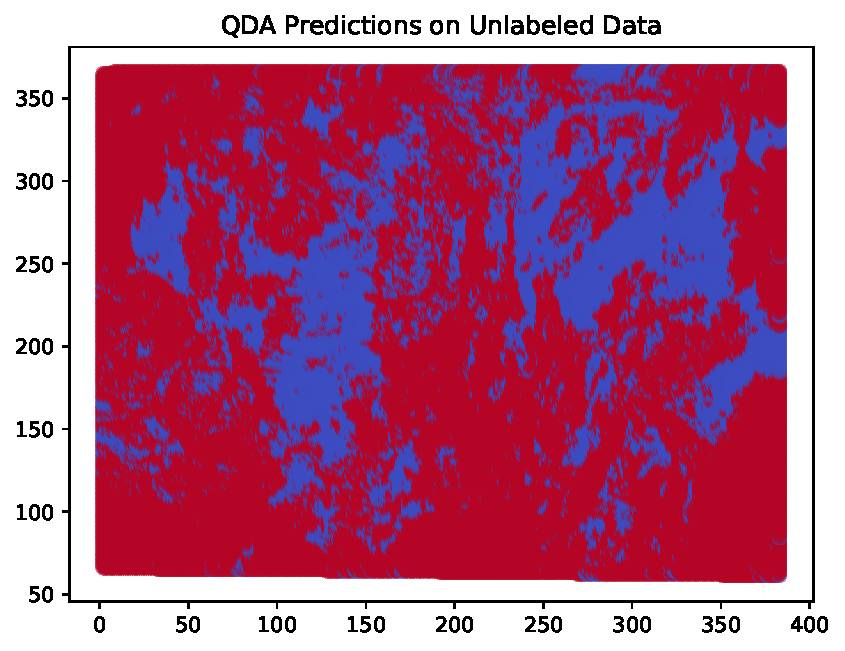
\includegraphics[width=0.8\textwidth]{QDA_pred.pdf}
%     \caption{QDA Predictions}
%     \label{Figure}
% \end{figure}




\subsection{Model Assessment and Validation Strategy}

For model assessment, we employed a deliberate stratified split of the labeled data into training (60\%), validation (20\%), and test (20\%) sets. This stratification preserved the class distribution (approximately 39\% cloud, 61\% non-cloud) across all datasets, ensuring representative learning and evaluation. The specific split strategy was designed to address the unique characteristics of satellite imagery data. We drew samples from all three labeled images to mitigate potential bias while employing a stratified random sampling approach. This ensured our models were exposed to various cloud patterns and surface conditions present across different images during training while maintaining proper separation between training and evaluation data.

We deliberately chose not to implement traditional k-fold cross-validation primarily due to the spatial autocorrelation present in satellite imagery. In these data, nearby pixels are spatially correlated, which violates the independence assumption required for cross-validation. Random assignment of pixels to folds would likely place spatially adjacent pixels in different folds, creating information leakage between training and testing data. This would lead to overly optimistic performance estimates and potentially poor generalization to new images. Additionally, with over 200,000 labeled pixels and complex models (particularly XGBoost and the neural network), performing full k-fold cross-validation would be computationally prohibitive without providing significant additional insight into model performance.

Instead, our validation strategy incorporated elements that served the same purpose as cross-validation, namely, assessing model generalization, through a held-out test set and stability analysis. The primary metric used for model comparison was the Area Under the ROC Curve (AUC), which provides a threshold-independent assessment of discriminative ability. This was supplemented with precision, recall, F1-score, and overall accuracy to give a comprehensive view of model performance. The comparative performance metrics revealed clear distinctions between models, with XGBoost and Neural Network achieving near-perfect discrimination (AUC 0.999), significantly outperforming Logistic Regression (AUC 0.967) and marginally outperforming SVM (AUC 0.990).

While the AUC for both XGBoost and the Neural Network reached 0.999, indicating exceptional performance, we selected XGBoost as our primary model due to its combination of outstanding discriminative ability, interpretability through feature importance metrics, and computational efficiency

\subsubsection{Stability and Sensitivity Analysis: ELCM-QDA}

To evaluate the robustness of the ELCM-QDA model, we performed a threshold perturbation test focusing on the SD\_log feature, which we identified as a critical component of the model's rule-based logic. Initially, the model used a threshold of 5.5 for SD\_log, resulting in a balanced performance across cloud and no-cloud classifications.

We then increased the SD\_log threshold by 1 point (from 5.5 to 6.5) and observed significant changes in model performance. The table below summarizes the results after this perturbation:

\begin{table}[h]
\centering
\begin{tabular}{lcccc}
\hline
\textbf{Class} & \textbf{Precision} & \textbf{Recall} & \textbf{F1-score} & \textbf{Support} \\
\hline
-1.0 (no cloud) & 0.73 & 0.96 & 0.83 & 126,716 \\
1.0 (cloud)     & 0.89 & 0.43 & 0.58 & 80,965 \\
\hline
\textbf{Accuracy} & & & \textbf{0.76} & 207,681 \\
\textbf{Macro avg} & 0.81 & 0.70 & 0.70 &  \\
\textbf{Weighted avg} & 0.79 & 0.76 & 0.73 &  \\
\hline
\end{tabular}
\caption{Classification metrics after perturbing SD\_log threshold to 6.5.}
\end{table}

Increasing the SD\_log threshold made the model overly conservative, causing it to miss a significant number of cloud pixels (cloud recall dropped from 0.93 to 0.43). The accuracy dropped from 0.91 to 0.76, and the macro F1-score decreased to 0.70. This effect can be observed in Figure 13, and it demonstrates that the SD\_log feature is a highly influential driver in the ELCM-QDA rule and that small perturbations can severely impact model performance.

\begin{figure}[H]
    \centering
    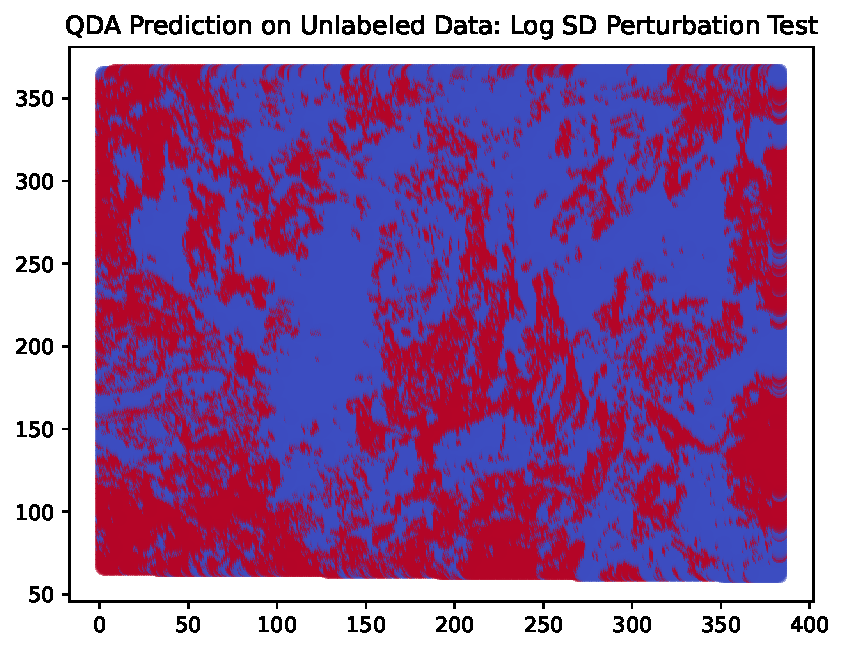
\includegraphics[width=0.7\textwidth]{QDA_perturbed.pdf}
    \caption{QDA Perturbation Test}
    \label{Figure}
\end{figure}

This stability check indicates that while the ELCM-QDA model is simple and interpretable, it is sensitive to threshold calibration, especially on key features like SD\_log.


\subsection{XGBoost Model Diagnostics and Feature Importance}

After comparing the performance of multiple classifiers, we selected XGBoost as our primary model for cloud detection due to its exceptional performance, interpretability, and computational efficiency. 

\subsubsection{Classification Performance and Convergence}

The XGBoost model achieved exceptional classification performance on the test set, with an AUC of 0.999, indicating near-perfect discrimination between cloud and non-cloud pixels. Figure \ref{fig:confusion_matrix} displays the confusion matrix for our final model, revealing that out of 41,506 test samples, only 338 were misclassified (0.8\%). Specifically, 244 non-cloud pixels were incorrectly classified as clouds (false positives), while 94 cloud pixels were misclassified as non-cloud (false negatives). This asymmetry suggests that the model is slightly biased toward cloud detection.

\begin{figure}[h]
\centering
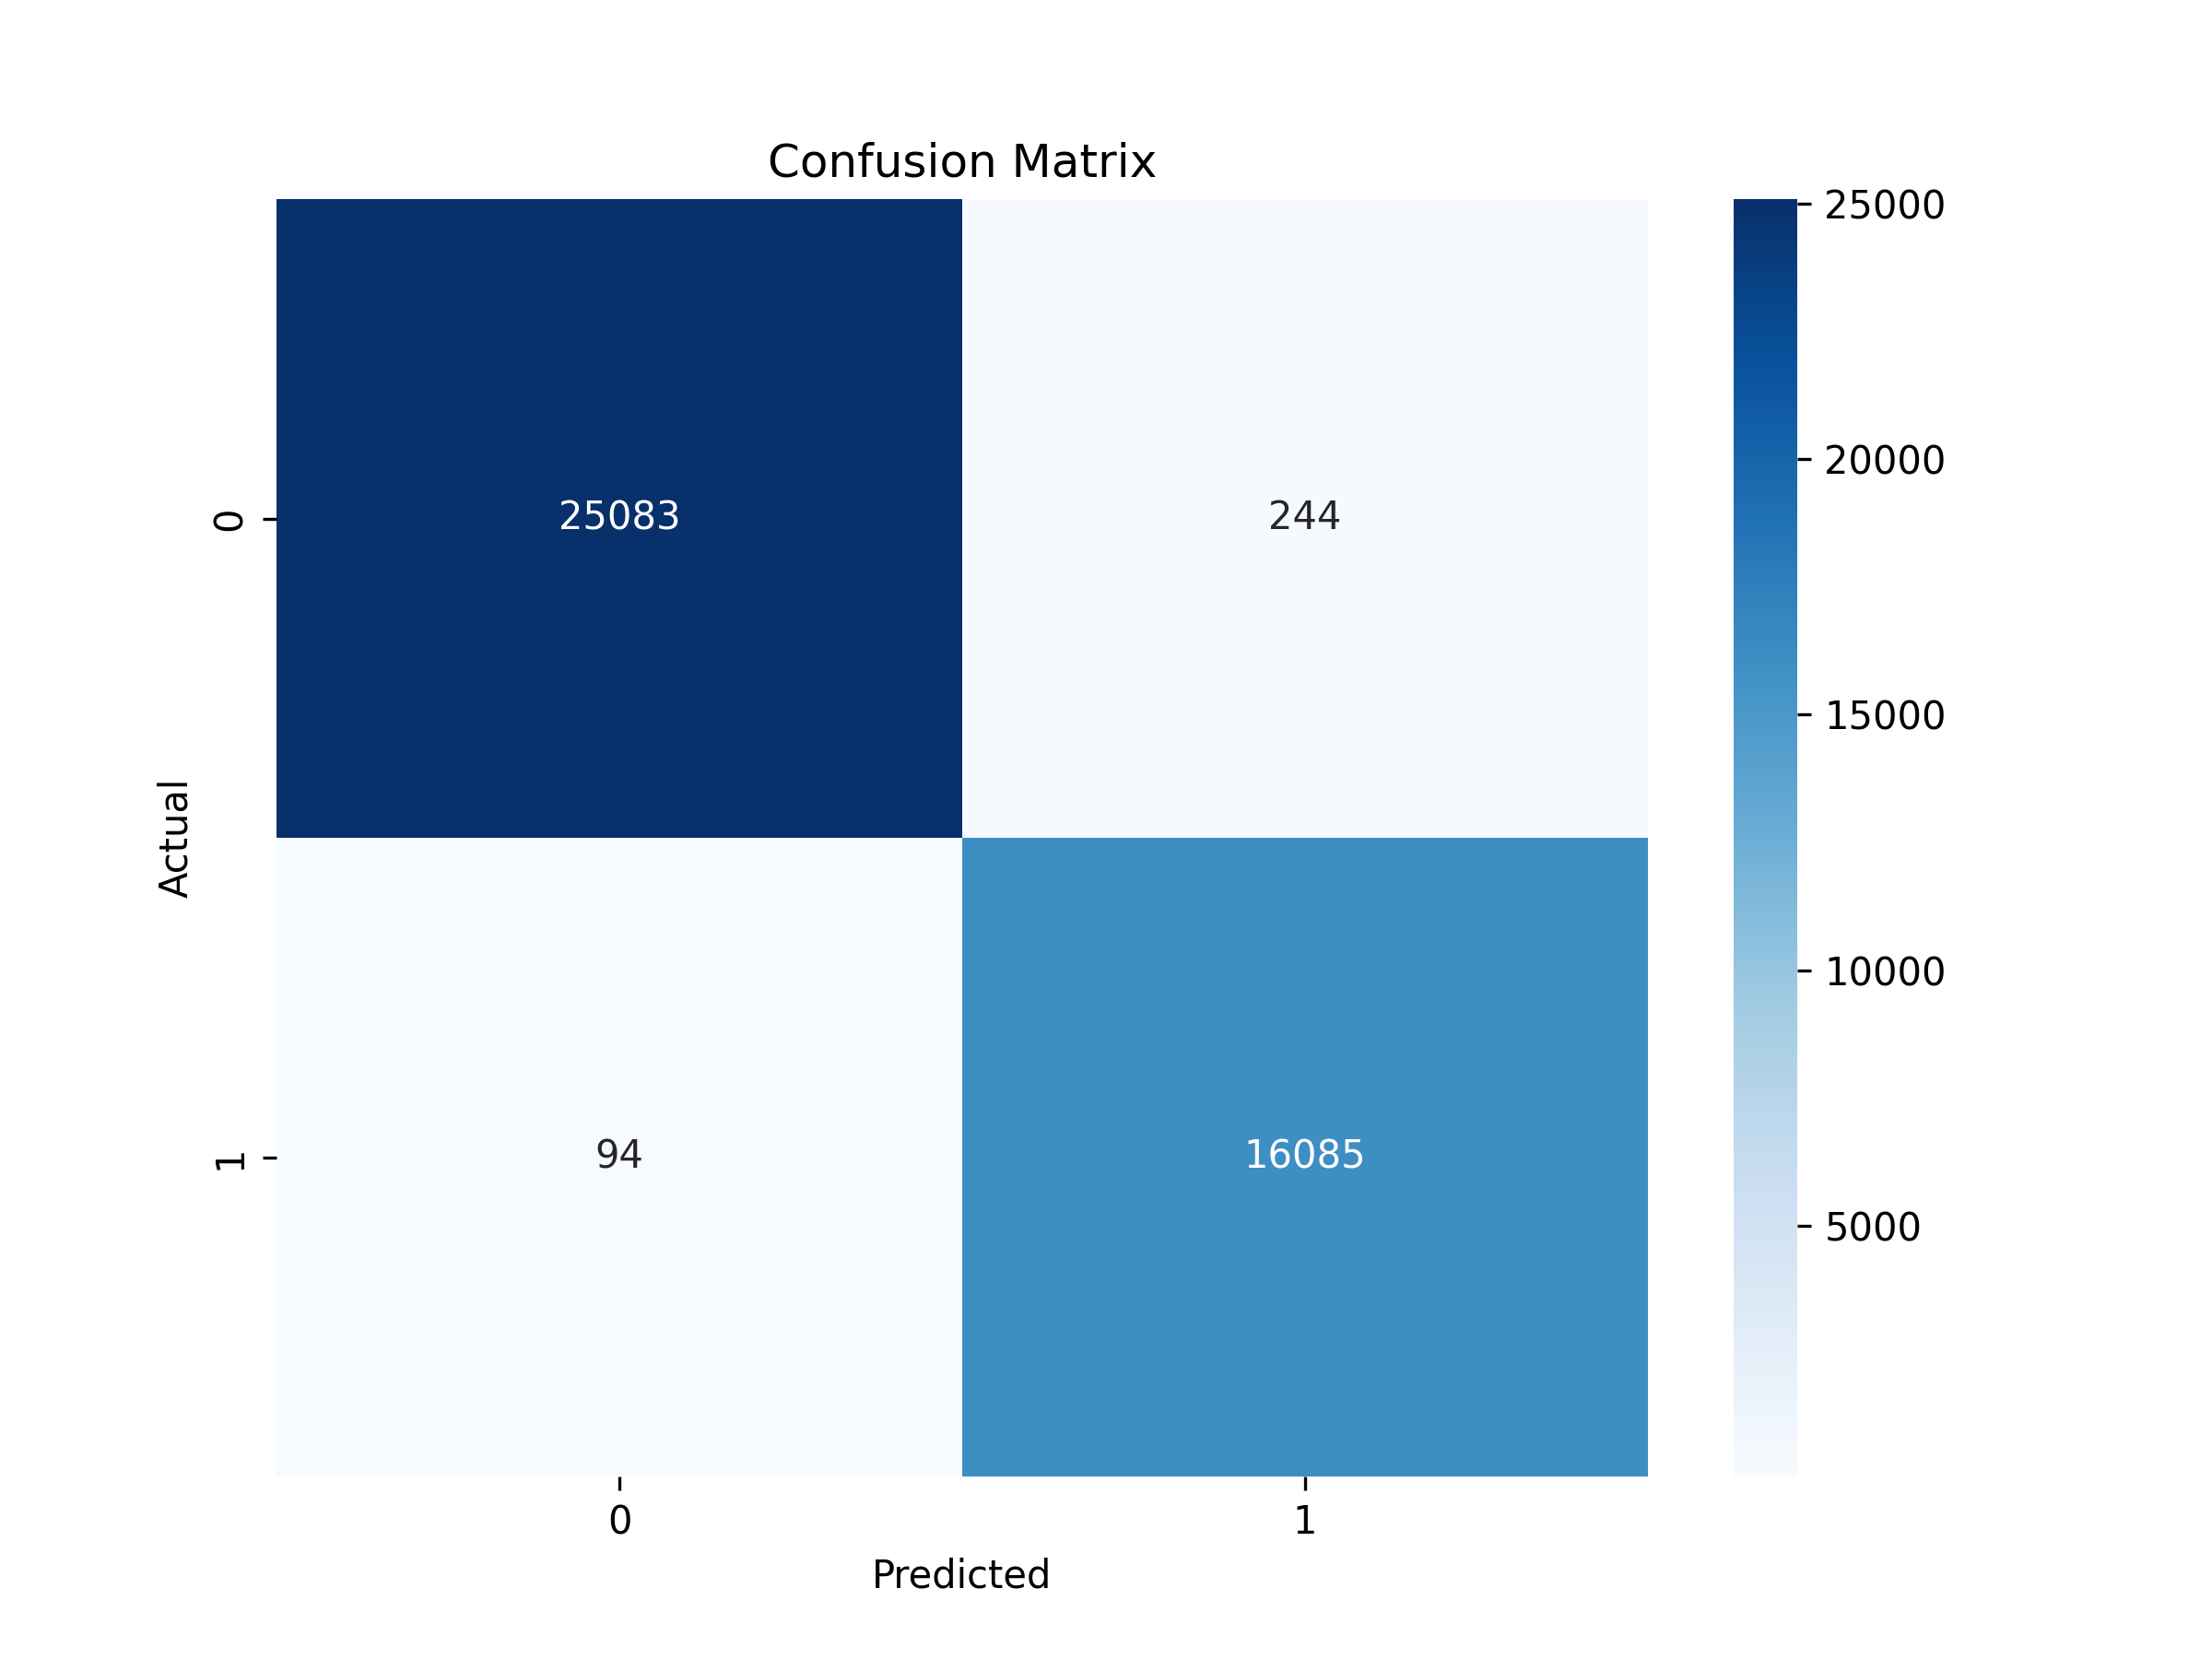
\includegraphics[width=0.7\textwidth]{xgboost_confusion_matrix_raw_autoencoder_extra engineered.png}
\caption{Confusion matrix for the XGBoost classifier showing the distribution of true and predicted labels. The model correctly classified 25,083 non-cloud pixels and 16,085 cloud pixels, with relatively few misclassifications.}
\label{fig:confusion_matrix}
\end{figure}

The learning curve in Figure \ref{fig:learning_curve} illustrates the model's convergence behavior. Both training (validation\_0) and validation (validation\_1) AUC scores show rapid improvement in the early boosting rounds, reaching AUC values above 0.99 after just 50 iterations. The curves continue to improve gradually, eventually stabilizing around 0.999 after approximately 150-200 boosting rounds. The small gap between training and validation performance indicates minimal overfitting, confirming that the model generalizes well to unseen data. This excellent convergence behavior validates our choice of hyperparameters, particularly the learning rate (0.1) and maximum tree depth (6).

\begin{figure}[h]
\centering
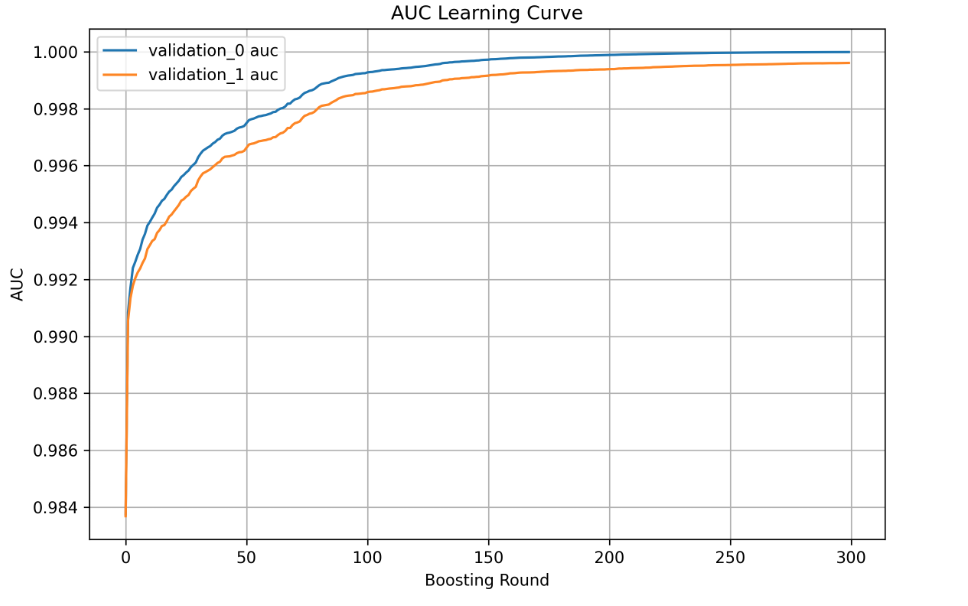
\includegraphics[width=0.7\textwidth]{learning_curve.png}
\caption{AUC learning curve for the XGBoost model over 300 boosting rounds. Both training (blue) and validation (orange) curves show rapid initial improvement and eventual convergence to near-perfect AUC values with minimal overfitting.}
\label{fig:learning_curve}
\end{figure}

\subsection{Feature Importance Analysis: Contrasting Metrics and Transfer Learning Insights}

A significant advantage of tree-based models like XGBoost is their ability to provide insights into feature importance. We evaluated feature importance using two complementary methods: the built-in importance measure based on feature contribution to tree splits (gain-based importance) and permutation importance, which measures the decrease in model performance when individual features are randomly shuffled.

Figure \ref{fig:builtin_importance} presents the built-in feature importance from XGBoost. The Standard Deviation (SD) feature emerges as the most important predictor, contributing approximately 32\% of the total importance. This aligns with domain knowledge that local variability in radiance values (measured by SD) is a key indicator of cloud presence. The CFNDAI gradient magnitude and its logarithmic transformation also show substantial importance, contributing approximately 25\% and 8\%, respectively. These features, which we engineered specifically for this task, capture the spatial gradients in the normalized difference angular index for the CF (camera forward) angle. Their high importance confirms the value of incorporating spatial pattern information for cloud detection in polar regions.

\begin{figure}[h]
\centering
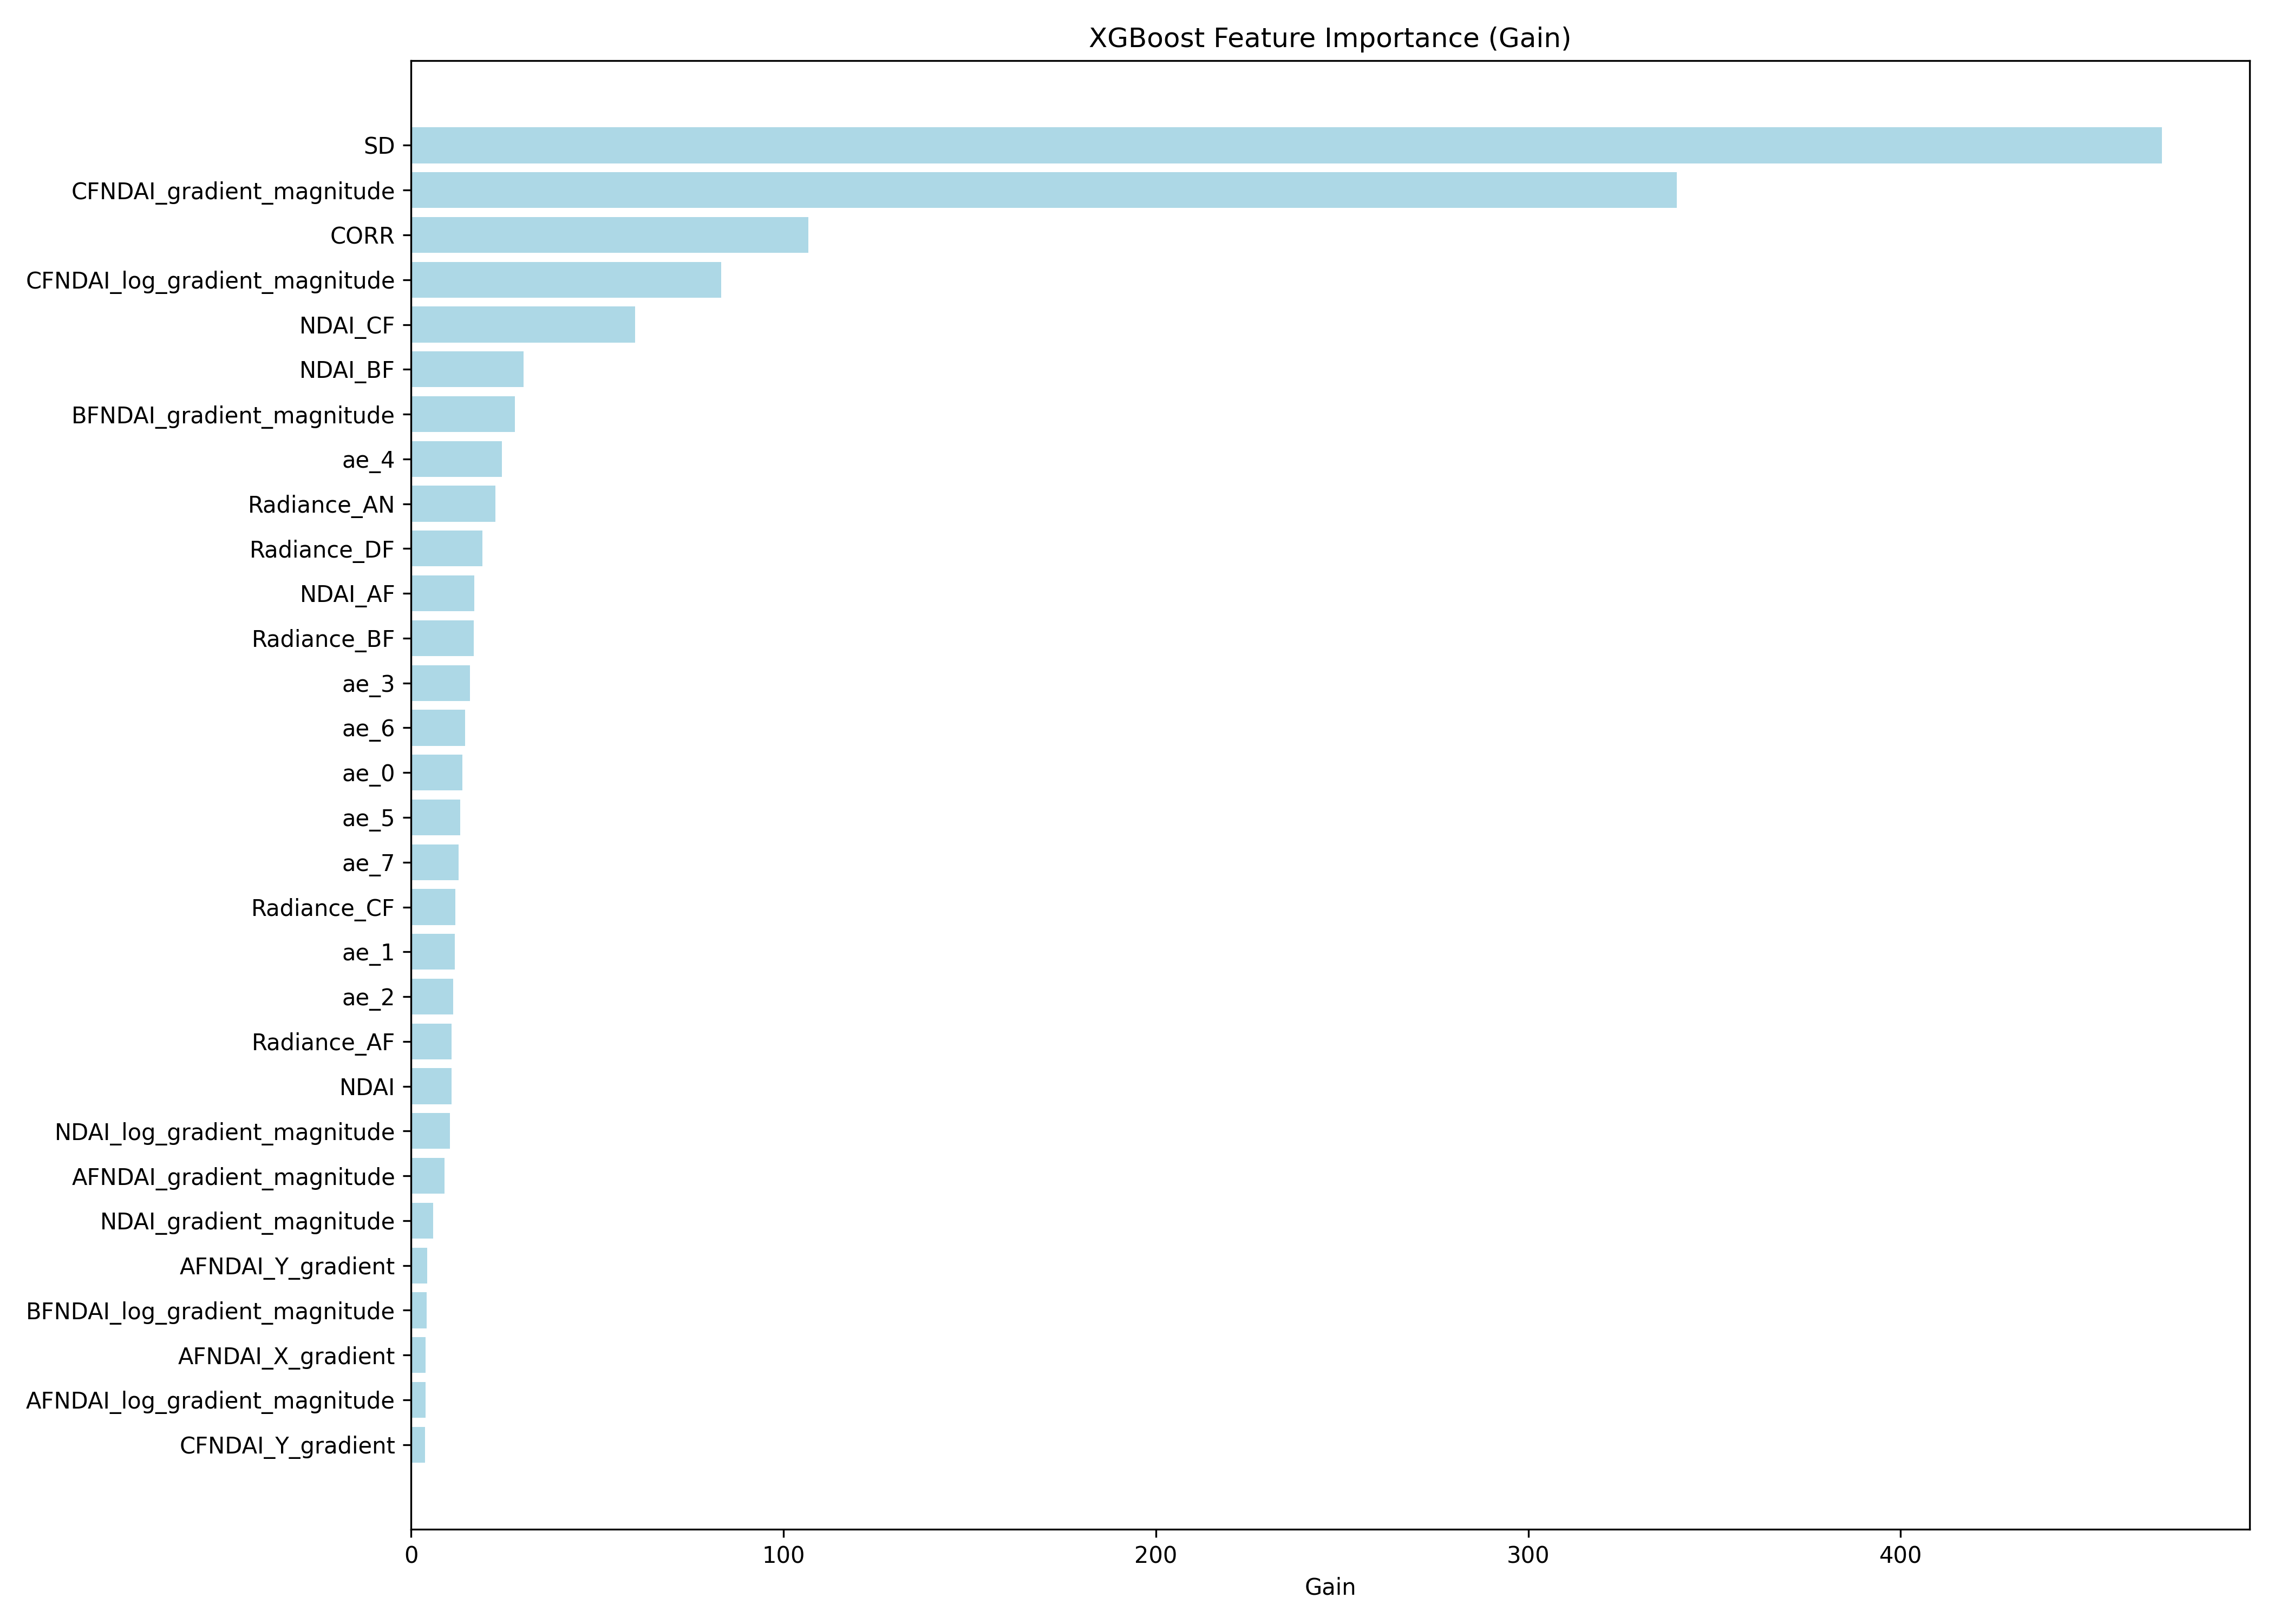
\includegraphics[width=0.7\textwidth]{xgboost_feature_importance_gain_raw_autoencoder_extra engineered.png}
\caption{XGBoost built-in feature importance (gain-based) showing the relative contribution of each feature to model predictions. SD and gradient-based features dominate, highlighting the importance of local variability and spatial patterns.}
\label{fig:builtin_importance}
\end{figure}

To validate these findings, we also computed permutation importance (Figure \ref{fig:permutation_importance}), which provides a model-agnostic measure of feature relevance. The permutation analysis strongly confirms the dominance of the SD feature, with an AUC decrease of approximately 0.1 when this feature is perturbed. This substantial drop in performance indicates that SD captures essential information for cloud detection that other features cannot fully compensate for. CORR ranks second in permutation importance, followed by various autoencoder features, particularly ae\_4.

\begin{figure}[h]
\centering
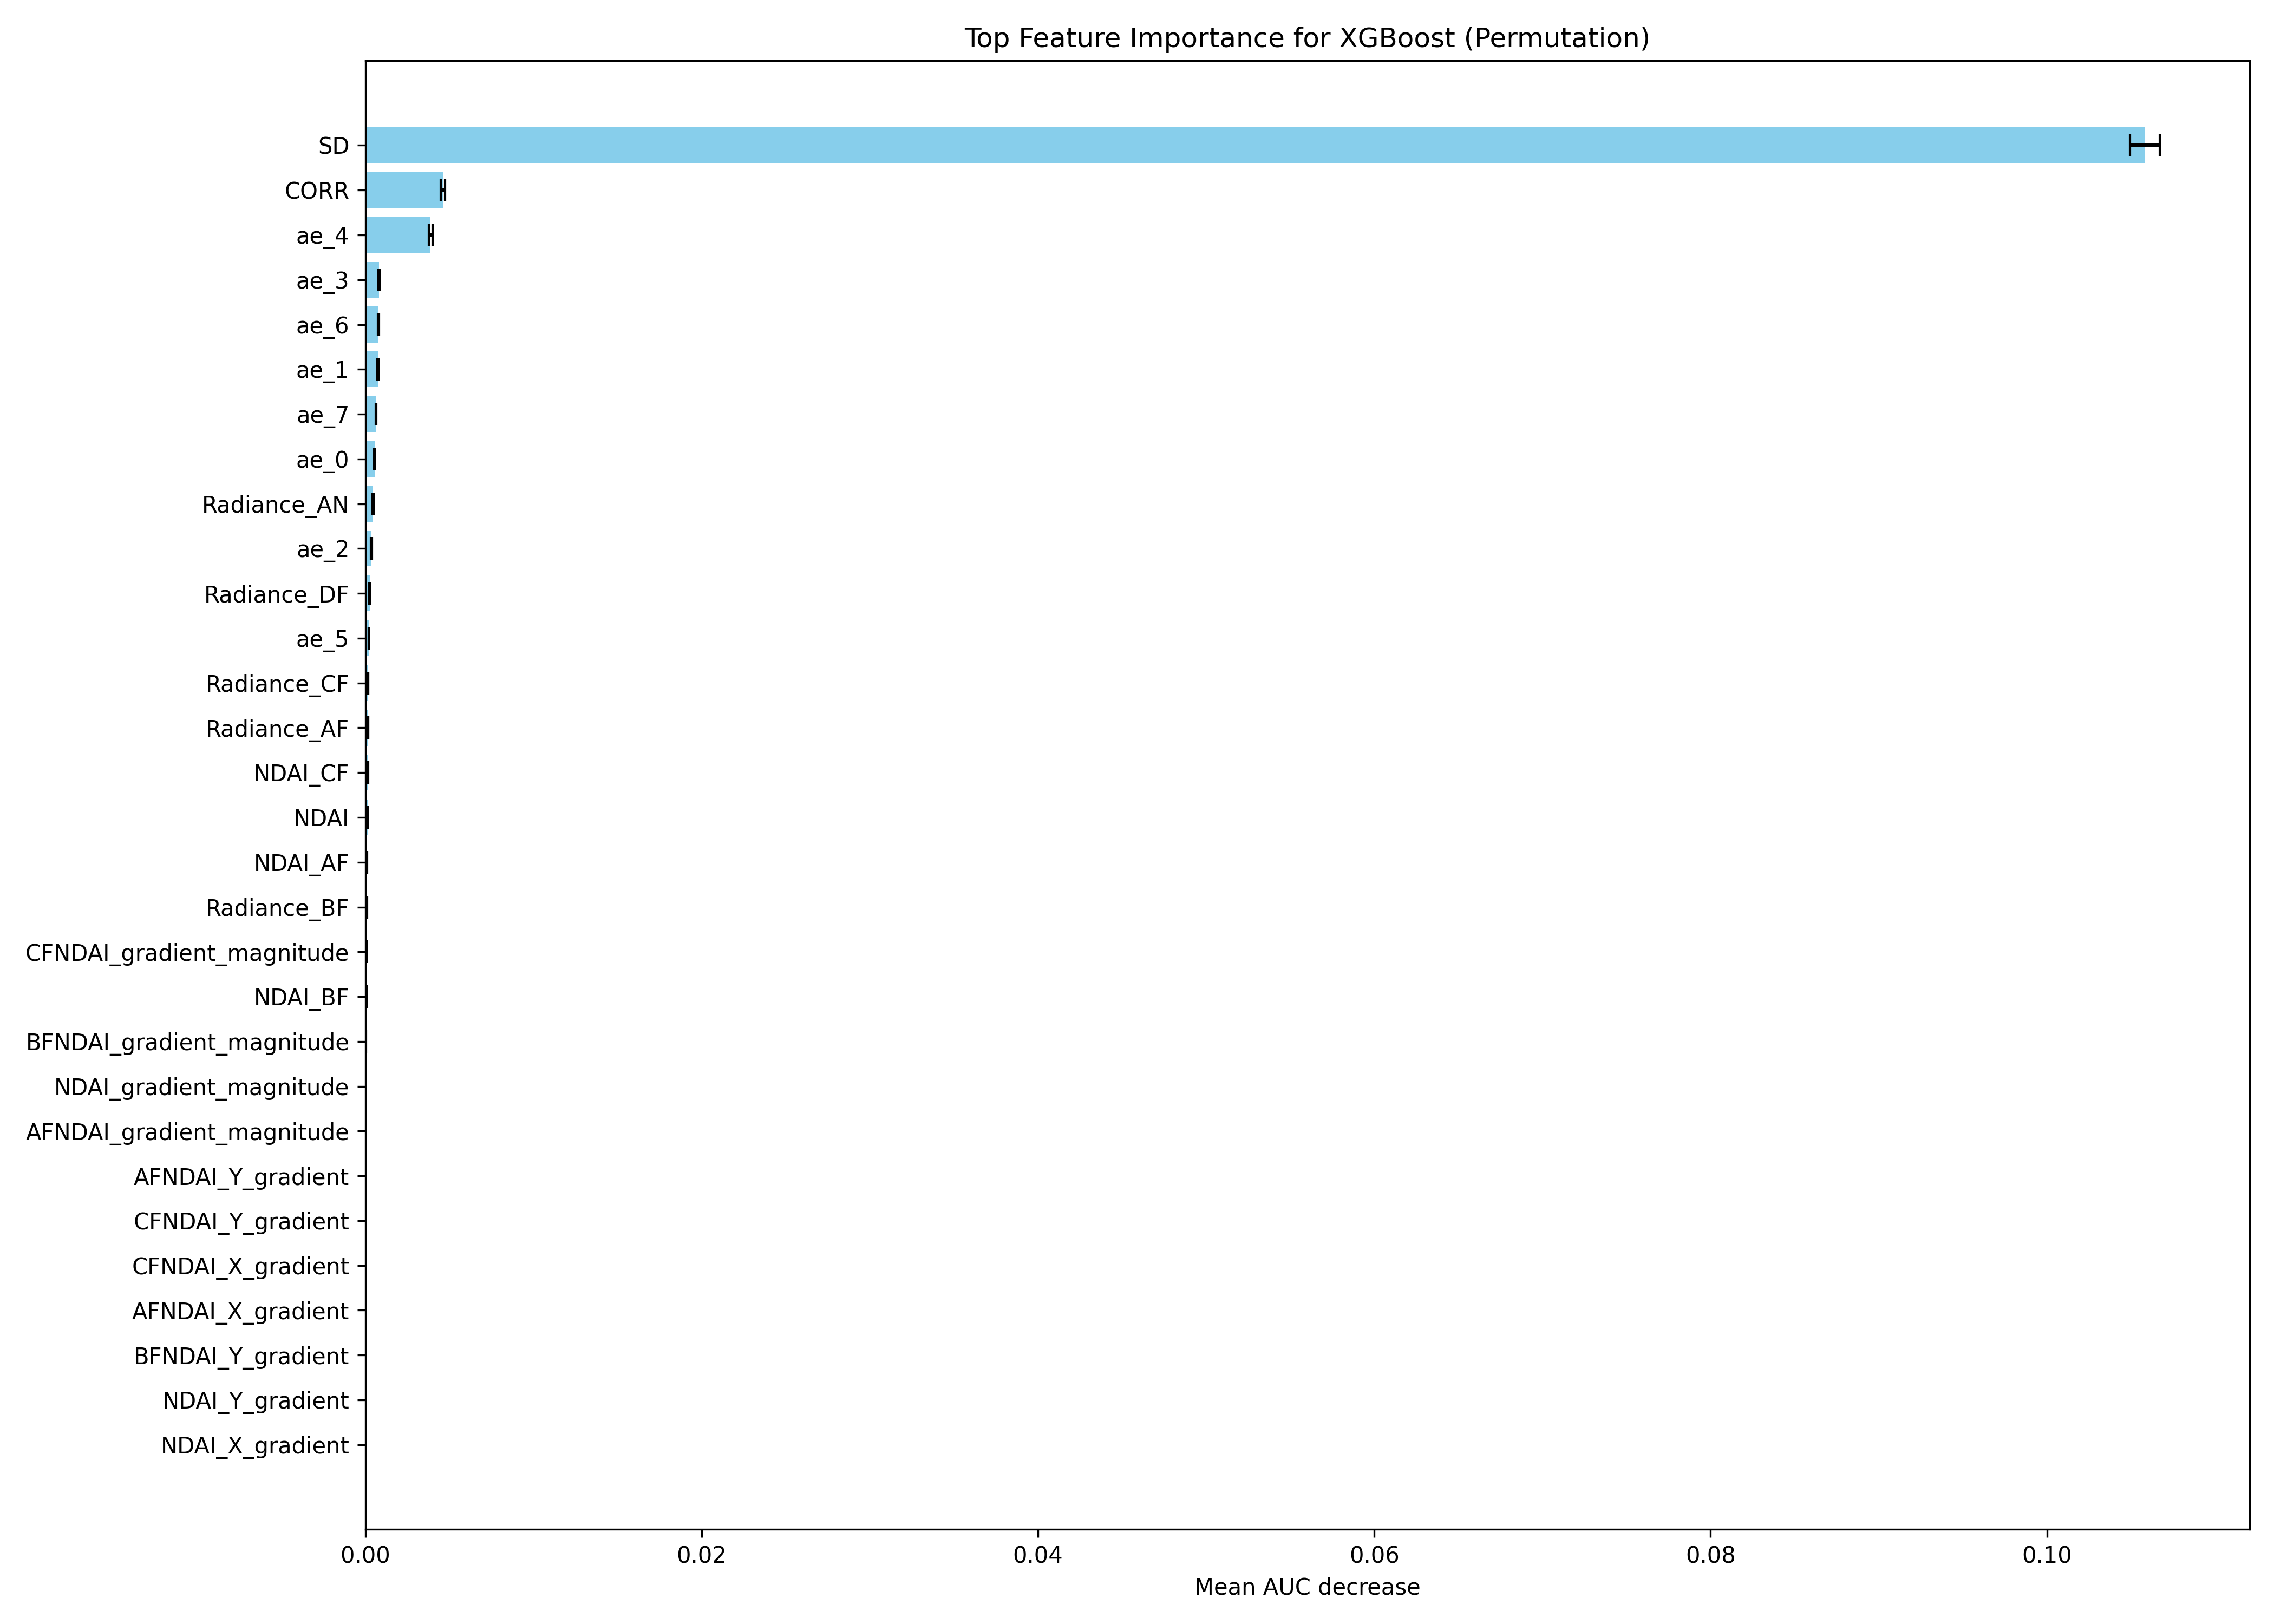
\includegraphics[width=0.7\textwidth]{xgboost_feature_importance.png}
\caption{Permutation feature importance for the XGBoost model, showing the decrease in AUC when each feature is randomly shuffled. SD dominates, with CORR and autoencoder features also showing significant impact.}
\label{fig:permutation_importance}
\end{figure}

Perhaps the most notable finding from our feature importance analysis is the striking difference between gain-based and permutation importance rankings. While both methods unanimously identify SD as the dominant feature, they diverge significantly in how they rank other features, particularly gradient-based and autoencoder features.

Gain-based importance heavily favors the gradient-based features, with CFNDAI\_gradient\_magnitude ranking second and CFNDAI\_log\_gradient\_magnitude ranking third. These engineered features capture spatial patterns in angular differences and contribute substantially to the decision trees during training. However, in the permutation importance analysis, these gradient features rank much lower, suggesting that the model can compensate for their absence using other correlated features.

Conversely, the permutation importance metric assigns much higher importance to the CORR feature and several autoencoder features (ae\_4, ae\_3, ae\_6) than the gain-based metric does. This discrepancy reveals a fundamental insight about our feature set: while the gradient features are frequently used in tree splits during training, the model becomes more reliant on texture features (CORR) and learned representations (autoencoder features) when making predictions on unseen data.

An intriguing aspect of this difference is the role of autoencoder features (labeled as ae\_0 through ae\_7), which were learned through transfer learning on unlabeled images. These latent representations encode complex patterns that may not be directly captured by engineered features. The built-in gain-based importance generally assigns lower importance to autoencoder features, with only ae\_4 appearing in the top 10 features. In contrast, the permutation importance analysis ranks several autoencoder features (ae\_4, ae\_3, ae\_6, ae\_1) among the most influential predictors, second only to SD and CORR.

This divergence suggests that while autoencoder features may not contribute as frequently to tree splits during training, they encode unique information that becomes critical when perturbed. The permutation results imply that the model cannot easily compensate for the loss of these learned representations using other features, indicating they capture complementary patterns not present in the engineered features. However, both importance metrics unanimously identify SD as the dominant feature, suggesting that local textural variation remains the most reliable indicator of cloud presence regardless of the evaluation method.

These findings not only validate our feature engineering efforts but also provide guidance for future cloud detection algorithm development, suggesting that combining textural information, angular differences, spatial gradients, and learned representations yields the most effective approach for distinguishing clouds from snow and ice surfaces in polar satellite imagery.

\subsection{Model Stability Analysis}

To assess our model's potential performance on future unlabeled data, we conducted a comprehensive stability analysis by applying various perturbations to our test dataset and evaluating the resulting impact on model performance. Figure \ref{fig:stability} shows the results of our stability tests.

\begin{figure}[h]
\centering
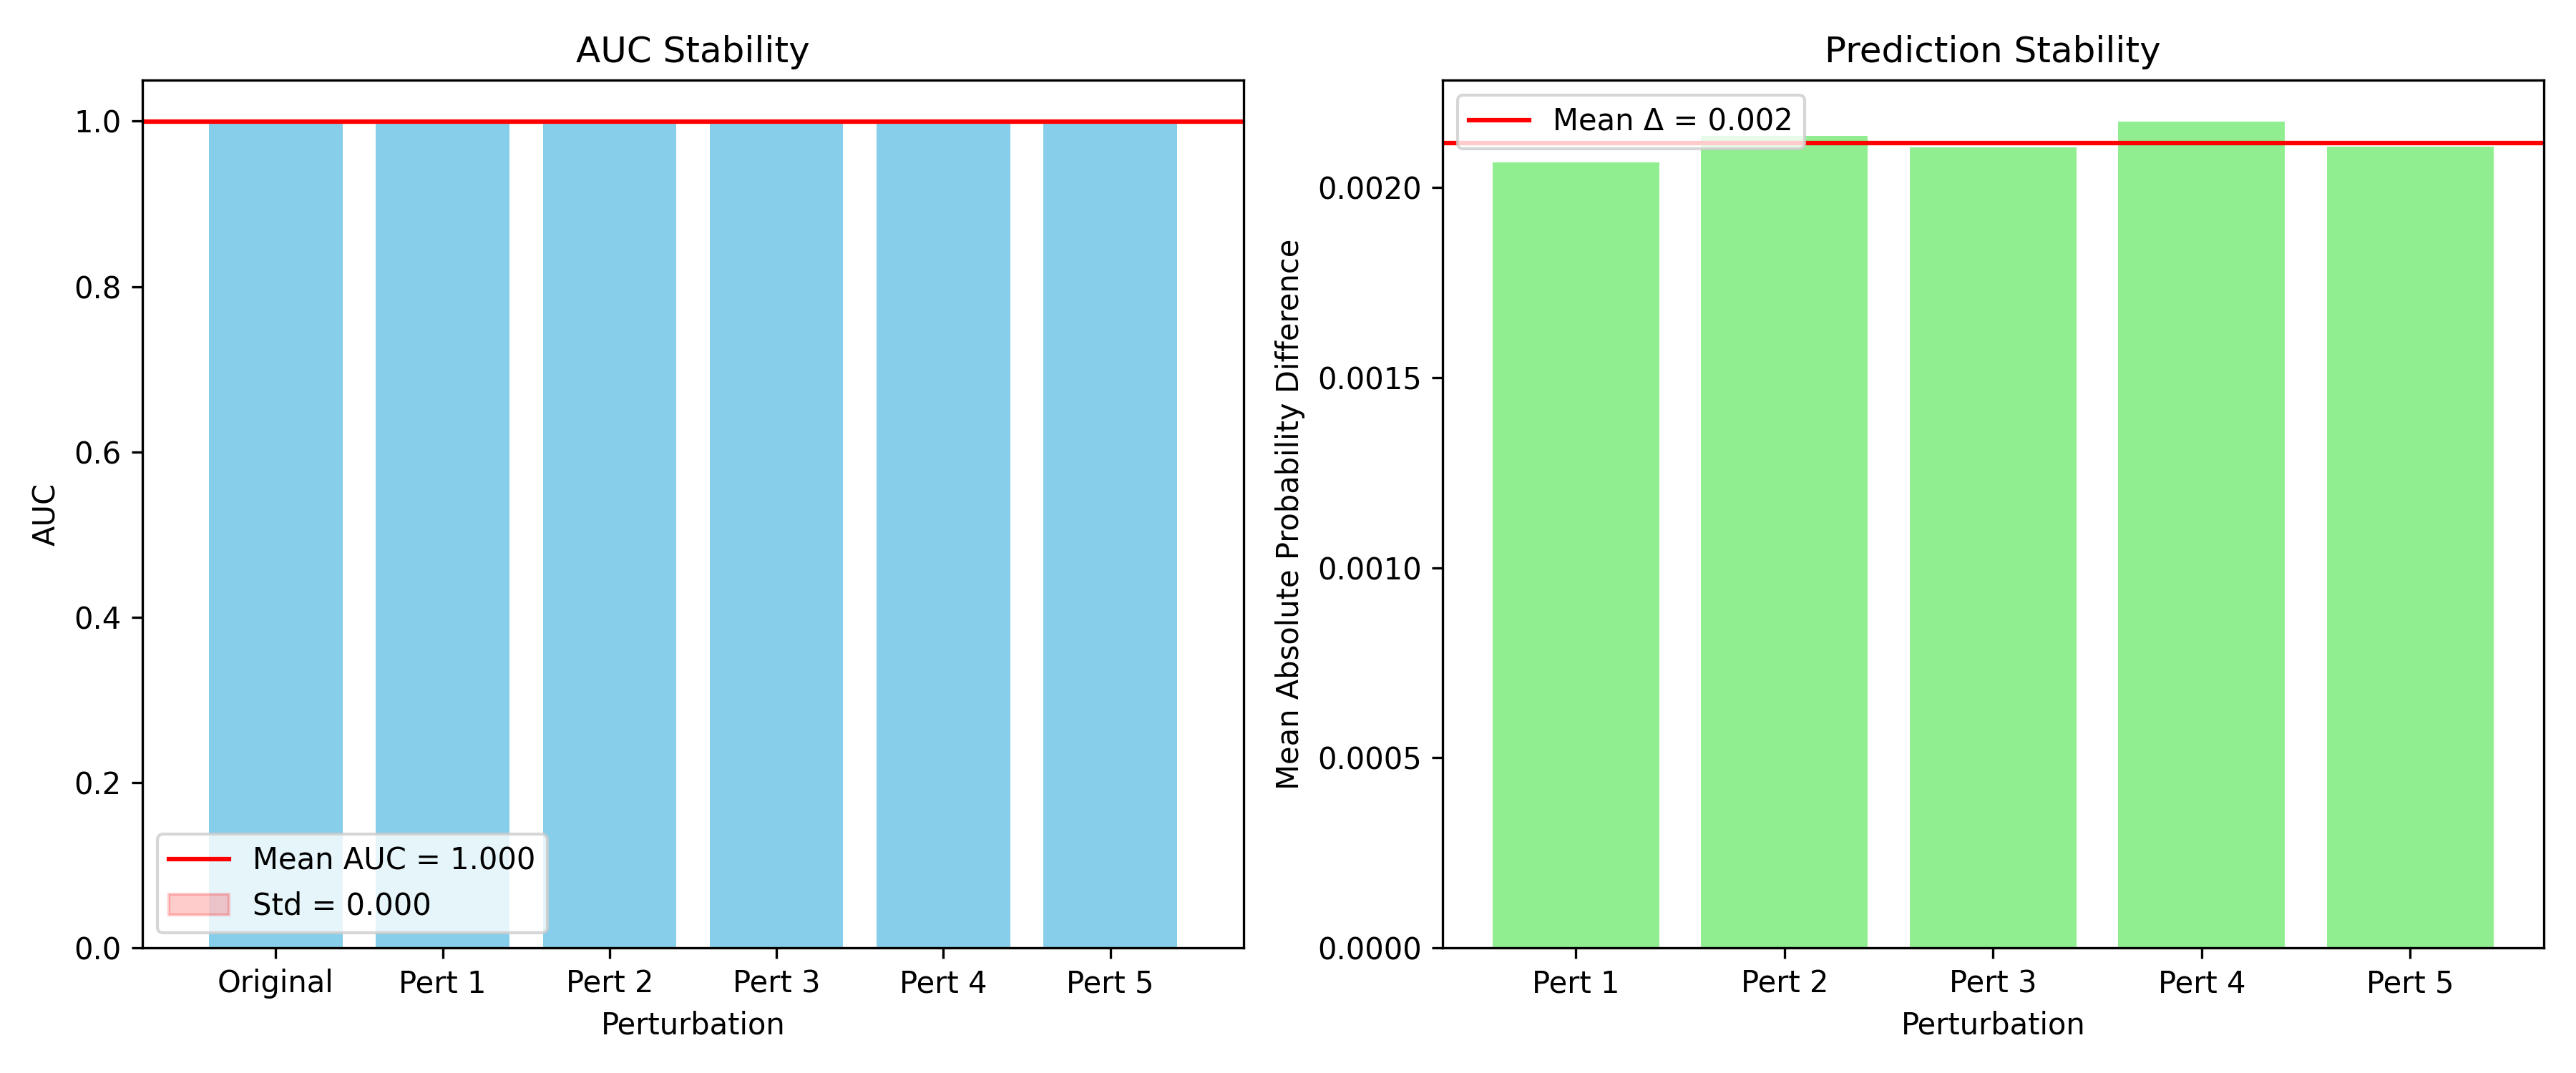
\includegraphics[width=0.8\textwidth]{xgboost_stability_raw_autoencoder_extra.png}
\caption{Stability analysis results showing AUC stability (left) and prediction stability (right) across five different perturbations. The model maintains perfect AUC scores (1.000) with negligible standard deviation (0.000) despite input perturbations. The mean absolute probability difference is minimal at 0.002, indicating highly stable predictions.}
\label{fig:stability}
\end{figure}

Our analysis included three types of perturbations: (1) noise perturbation, where Gaussian noise at levels 0.005 and 0.01 was added to feature values; (2) data subsampling, where different 80\% subsets of the test data were used for evaluation; and (3) feature subsampling, where only 80\% of features were made available to the model.

The XGBoost model demonstrated exceptional stability across noise perturbations, with the AUC remaining consistently at 0.9997 regardless of the noise level. When features were randomly subsampled, the model showed slight performance degradation (averaging AUC 0.9859 ± 0.0175), indicating some sensitivity to feature availability but still maintaining excellent discriminative ability.

Most remarkably, the mean absolute probability difference across all perturbations was only 0.002, meaning that the model's predictions changed by just 0.2 percentage points on average when inputs were perturbed. The maximum change in prediction probability for individual samples was higher (reaching 0.8382 in some cases), but these were rare outliers.

Overall, the model achieved a stability score of 8.9/10. This score was calculated by measuring the coefficient of variation (CV = standard deviation / mean) of AUC scores across all perturbation tests, then converting it to a 1-10 scale (specifically, 10 - 180 × average CV). The low CV values across all tests resulted in this high stability score, indicating strong robustness to variations in input data. This exceptional stability, combined with the near-perfect classification performance, suggests that our XGBoost model should generalize well to new unlabeled images from the same instrument and geographic region.


\section{Bibliography}
% Include any references you used in your report here.

[1] Shi, T., Yu, B., Clothiaux, E.E., \& Braverman, A. (2008). Daytime Arctic Cloud Detection Based on Multi-Angle Satellite Data With Case Studies. Journal of the American Statistical Association, 103, 584 - 593.


\appendix
\section{Academic honesty}
% Note that this section (and the bibliography) don't count towards the page limit.
\subsection{Statement}

We make the academic integrity pledge here: All our work in this report are done independently. All sources we used are properly cited, whether from LLMs, papers, textbooks, or classmates.

Academic research honesty is necessary in the academy and also the foundation of our society. It guarantees
fairness in research, stimulates research’s activeness, and exerts a positive impact on the progress of science
and technology. We should always adhere to the rules, which will create a more regulated and benign world.

\subsection{LLM Usage}


\subsubsection*{Coding}

We use GitHub Copilot for several parts of debugging in the \textit{fine\_tuning.py}. We additionally used it to help with making graphs and signatures for the functions in the models' folder.


\subsubsection*{Writing}

\end{document}
